\documentclass[a4paper,12pt]{book}

\usepackage[english]{babel}
\usepackage[utf8]{inputenc}
\usepackage[T1]{fontenc}

\usepackage{textcomp}
\usepackage{newlfont}
\usepackage{color}

\textwidth=450pt\oddsidemargin=0pt


\usepackage{emptypage}
 % remove header in blanck pages

% caption style
\usepackage{caption}
\usepackage{subcaption}
\captionsetup[figure]{labelfont=bf,textfont=it}
\captionsetup[table]{labelfont=bf,textfont=it}

% figure numeration
%\usepackage{chngcntr}
%\counterwithin{figure}{chapter}
%\counterwithin{figure}{section}
\usepackage[a4paper,top=3cm,bottom=2cm,left=3cm,right=3cm,marginparwidth=1.75cm]{geometry}


%useful packages
\usepackage{amsmath} % mathematics
\usepackage{amssymb} % mathematics
\usepackage{graphicx}
\usepackage[ruled,vlined]{algorithm2e} % pseudocode
\usepackage{multirow}
\usepackage{hyperref}



% include file and not recompile it
\usepackage{standalone}
\usepackage{dsfont}

\usepackage{listings}

\definecolor{codegreen}{rgb}{0,0.6,0}
\definecolor{codegray}{rgb}{0.5,0.5,0.5}
\definecolor{codepurple}{rgb}{0.58,0,0.82}
\definecolor{backcolour}{rgb}{0.95,0.95,0.92}

\lstdefinestyle{python}{
	backgroundcolor=\color{backcolour},
	commentstyle=\color{blue}\ttfamily,
	keywordstyle=\color{green}\ttfamily,
	numberstyle=\tiny\color{magenta},
	stringstyle=\color{red}\ttfamily,
	basicstyle=\ttfamily\footnotesize,
	morecomment=[l][\color{magenta}]{\#}
	breakatwhitespace=false,
	breaklines=true,
	captionpos=t,
	keepspaces=true,
	numbers=left,
	numbersep=5pt,
	showspaces=false,
	showstringspaces=false,
	showtabs=false,
	tabsize=2
}

% figures
%\usepackage{subfigure}
%bibliografia
\usepackage[backend=biber,style=numeric,autocite=plain,sorting=none]{biblatex}
% include file and not recompile it


\graphicspath{{img/}}
\addbibresource{bibliography.bib}



\begin{document}


\begin{titlepage}
%
%
% ONCE YOU ARE FINISHED WITH YOUR CHANGES MODIFY "RED" WITH "BLACK" IN ALL \textcolor COMMENTS
%
%
\begin{center}
{{\Large{\textsc{Alma Mater Studiorum $\cdot$ University of  Bologna}}}} 
\rule[0.1cm]{15.8cm}{0.1mm}
\rule[0.5cm]{15.8cm}{0.6mm}
\\\vspace{3mm}
{\small{\bf School of Science \\
Department of Physics and Astronomy\\
Master Degree in Physics}}
\end{center}

\vspace{23mm}

\begin{center}\textcolor{black}{
%
% INSERT THE TITLE OF YOUR THESIS
%
{\LARGE{\bf Automatic Pipeline for the Identification of Ground Glass Opacities on CT Images of Patients Affected by COVID-19}}\\
}\end{center}

\vspace{50mm} \par \noindent

\begin{minipage}[t]{0.47\textwidth}
%
% INSERT THE NAME OF THE SUPERVISOR WITH ITS TITLE (DR. OR PROF.)
%
{\large{\bf Supervisor: \vspace{2mm}\\\textcolor{black}{
Prof. Gastone Castellani}\\\\
%
% INSERT THE NAME OF THE CO-SUPERVISOR WITH ITS TITLE (DR. OR PROF.)
%
% IF THERE ARE NO CO-SUPERVISORS REMOVE THE FOLLOWING 5 LINES
%
\textcolor{black}{
\bf Co-supervisor:
\vspace{2mm}
Dr. Nico Curti\\\\}}}
\end{minipage}
%
\hfill
%
\begin{minipage}[t]{0.47\textwidth}\raggedleft \textcolor{black}{
{\large{\bf Submitted by:
\vspace{2mm}\\
%
% INSERT THE NAME OF THE GRADUAND
%
\textcolor{black}{
Riccardo Biondi}}}
}
\end{minipage}

\vspace{40mm}

\begin{center}
%
% INSERT THE ACADEMIC YEAR
%
Academic Year \textcolor{black}{ 2019/2020}
\end{center}

\end{titlepage}


\thispagestyle{empty}
\pagenumbering{gobble}
\documentclass{standalone}
\begin{document}

	\chapter*{Abstract}\addcontentsline{toc}{chapter}{Abstract}
	\markboth{Abstract}{Abstract}
	
	COronaVirus Disease (COVID-19) has widely spread all over the world since the beginning of 2020. It is acute, highly contagious, viral infection mainly involving the respiratory system.

	Chest CT scans of patients affected by this condition have shown peculiar patterns of Ground Glass Opacities (GGO) and Consolidation (CS) related to the severity and the stage of the disease.

	In this scenario, the correct and fast identification of these patterns is a fundamental task. Up to now this task is performed mainly using manual or semi-automatic techniques, which are time-consuming (hours or days) and subjected to the operator expertise.

	In this work of thesis, I have developed and implemented an automated pipeline for the identification of GGO and CS patterns in chest CT scans. To achieve this purpose, I have applied colour quantization and obtained a hard classification based on voxel intensities. I have used the way in which digital images encodes colour to takes into account also properties related to the voxel neighbourhood, useful since lesions involve many close voxels.
	
	The pipeline was tested on three different datasets and compared with manual annotation by checking specificity and sensitivity and with a blind evaluation made by experts. The results of these preliminary tests show that the pipeline is able to achieve segmentation with high specificity in less than $3\,min$. Even if the total lesion volume is underestimated, the pipeline has shown to achieve segmentation consistent with annotation. 


	
\end{document}


\pagenumbering{gobble}
\tableofcontents

\thispagestyle{empty}
\pagenumbering{arabic}
\documentclass{standalone}
\begin{document}

\chapter*{Introduction}\addcontentsline{toc}{chapter}{Introduction}
\markboth{Itroduction}{Introduction}


Since the end of 2019, COVID-19 has widely spread all over the world.Up to now the gold standard for the diagnosis of this disease are the reverse transcription-polymerase chain reaction (RT-PCR) and the gene sequencing of sputum, throat swab and lower respiratory tract secretion~\cite{ART:Zhao}.\\ Many COVID-19 affected patients have shown ground glass opacities(GGO) and consolidation(CS) in chest CT,for which the severity, shaoe and involved of lung parenchima are made in relation with the stage of the disease ~\cite{ART:Bernheim}.  As shown by \cite{ART:Huang}, initial prospective analysis have shown that the $98\%$ have bilateral patchy shadows or ground glass opacity (GGO) and consolidation(CS) in lung. Other study have have monitored the change on volume and shape of these features on healed patients~\cite{ART:Ai} in order to monitoring their recovery. In \figurename\,\ref{fig:HealthVSCovid} are compared slices of an healthy control and a patient affected by COVID-19. We can clearly see the GGO and CS regions in the lung of the second one from left.\\
	
\begin{figure}[h!]
	\centering
	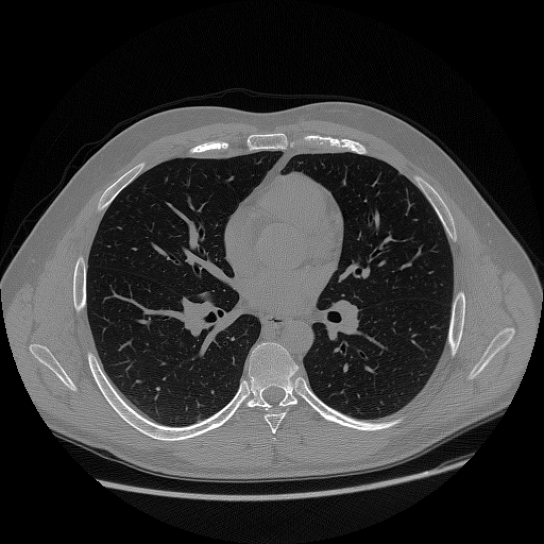
\includegraphics[scale=.5]{healthy.png}
	\quad
	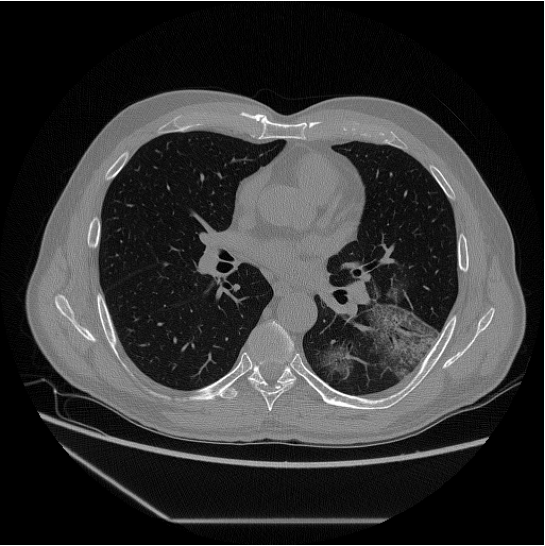
\includegraphics[scale=.5]{ggo.png}
	\label{fig:HealthVSCovid}\caption{CT scan of thorax for an healthy patient(left) and a COVID-19 affected one(right) in which we can observe a huge amount of GGO in the right lung}
\end{figure} 


GGO and CS are not exclusive of COVID-19, but may be also caused by pulmonary edema, bacterial infection, other viral infection or alveolar haemorrage~\cite{ART:Collins}. However the combination between CT scan information and other diagnostic techniques like the RT-PCR mentioned above, may help the diagnosis, the monitoring of the course of the disease and the checking of the recovery in healed patients. The study of these patterns may help to understand the infection pathogenesis, which is not well known since COVID-19 is a new disease.\\
Austin in Glossary of terms for CT of the lungs~\cite{ART:Austin} define the Ground Glass Opacities as \emph{hazy increased attenuation of lung, with preservation of bronchial and vascular margins caused by partial filling of air spaces, interstitial thickening, partial collapse of alveoli, normal expiration, or increased capillary blood volume}.
For the reason given before, the identification of this kind of lesions in CT scans of lung is very important. Up to now the segmentation is made in a manual or semiautomatic way, which are time consuming and subjective, since involves the interaction with trained personnel. An automatic and fast way for the identification of this features is desired.\\
In this thesis work I will present an automatic and fast pipeline for the identification of these kind of lesions. The pipeline was developed by using $83$ chest CT scans of COVID-19 affected patients, kindly provided by Sant'Orsola hospital. Also scans from two public dataset (ZENODO~\cite{DATA:ZENODO}, MOSMED~\cite{DATA:MOSMED}) are used as benchmark.\\
The developed pipeline is completely unsupervised and its based on the color quantization, so the relation between the HU and the different linear attenuation coefficient of tissues is exploited. In order to takes into account other features, like the spatial extension of the lesion areas, or the different shape of the lung structure, a suitable color space was build.\\
The pipeline was implemented in python and to perform the different operations different image processing libraries where used : \emph{SimpleITK}, \emph{OpenCV} and \emph{scikit-image}.\\
The time performance of the pipeline are verified on the DIFA servers and the segmentation accuracy on labels provided by the manual segmentation performed by experts.

\end{document}


\documentclass{standalone}
\begin{document}
	
	\documentclass{standalone}
\begin{document}
\chapter{Image Segmentation techniques}
	Image segmentation consists of the partitioning of an image into non-overlapping consistent regions that are homogeneous respect to some characteristics, such as intensity or texture~\cite{ART:Pham}.
	The results of segmentation can be used to perform feature extraction, that provides fundamental information about organs or lesion volumes, cell counting, etc. If a patient performs many analysis during the time, image segmentation is a useful tool to monitor the evolution of particular lesions or tumours during therapy.
	Nowadays different non-invasive medical imaging techniques are available, such as Computed Tomography (CT), Magnetic Resonance Imaging (MRI) or X-Ray imaging, that provide a map of the subject anatomy or function. 
	
	Image segmentation plays a crucial role in many medical imaging applications by automating or facilitate the delineation of anatomical structures and other regions of interest~\cite{ART:Pham}.  Manual segmentation is possible, but it is time-consuming and subject to operator variability making the results difficult to reproduce~\cite{INP:Withey}. Therefore automatic or semi-automatic methods are preferable. 
	
	The major difficulty in medical image segmentation is the high variability in medical images. First and foremost, human anatomy itself shows major modes of variation~\cite{ART:Pooja}. Furthermore, the many different modalities (X-ray, CT, MRI, etc.) used to create medical images change the particular meaning of the data.
	
	In this chapter I will provide a brief introduction about medical images, focusing mainly on Computed Tomography, which is the technique used to acquire the images segmented in this work. 	
	This part is followed by a discussion on the main image segmentation techniques.
	
\end{document}
	
	\documentclass{standalone}
\begin{document}
	\section{Medical Images}
	
	A medical image is the representation of the internal structure or function of the anatomic region in the form of an array of picture elements (pixels/voxels). 
	This discrete representation result from a process that maps each numerical value in a position of the space. The number of pixels used for this representation is an expression of the details with which the anatomy of function can be depicted. The physical meaning of the data changes according to the image acquisition modality (CT, MRI, PET, etc.); for instance, we can consider the computed tomography (CT) case: 
	
	Computed Tomography (CT) is a medical imaging technique which aims to reproduce cross-section images and the 3D anatomy of the examined subject. Each data represents the capability of the corresponding volume to attenuate an x-ray beam. To match results from different scans, the beam attenuation is measured in Hounsfield Units(HU) : 
	\begin{equation}\label{eq:HU}
		CT-number = 1000\times\frac{\mu - \mu_{H_2O}}{\mu_{H_2O}}
	\end{equation}
	Where $\mu$ is the linear attenuation coefficient of the tissue, $\mu_{H_20}$ is the linear attenuation coefficient of the water, took as a reference. The linear attenuation coefficient of the air is considered as $0$, so the corresponding CT number is $-1000$. For the bones, that have a density double than water, the CT number is $1000$.
	
	Medical images can be characterized by $5$ properties: \emph{pixel depth, photometric, interpretation, metadata and pixel data}. 
	
	\paragraph*{Pixel depth} Pixel Depth is the number of bits used to encode the information of each pixel. Each value of the tensor is an integer of floating-point number belonging to a domain related to the image format. It is related to the memory space necessary to store the image and the amount of information we want to store in each pixel. Higher bit allows us to store more information but requires more memory~\cite{ART:Larobina}. The most common are $[0, 255]$ for $8-$bit integer image, of $[0, 1]$ for floats. Also, other formats are available, like $16-$bit integers, widely used to represent medical images. 
	
	\paragraph{Photometric Interpetation} The photometric interpretation specifies how the pixel data should be interpreted for the correct image display as a monochrome or colour image. We have to introduce the concept of \emph{number of channels}. Monochrome images have only one sample per pixel (GL intensity). To encode colour information into pixels, we typically need multiple samples per pixel and to adopt a colour model that specifies how to obtain colours combining the samples. Colour may be used to encode blood flow direction and velocity in Doppler ultrasound~\cite{ART:Larobina}. In this works, I have used colour to consider also voxels neighbouring information and different image gamma 
	
	\paragraph{Metadata} 
	Metadata are the information that describes the image. Metadata is typically stored at the beginning of the file and contains (at least) the image matrix dimension and photometric interpretation. In medical image formats, it contains also information about how the image was produced or about the patients~\cite{ART:Larobina}.
	
	\paragraph{Pixel Data} Numerical values of the pixels that are stored according to data type. 
			
\end{document}
	\documentclass{standalone}
\begin{document}
	\subsection{Medical Image Formats}
	
	Image file formats provide a standard way to store the information describing an image in a computer file. Moreover file format  describes how the image data are organized inside the image file and how the pixel should be interpreted by a software for the correct loading and visualization.
	
	Medical file formats can be divided in two categories: one that try to standardize the images generated by diagnostic modality(e.g. DICOM), the other that try to facilitate the post processing analysis (e.g. Nifti). Both of them stores image data and metadata at the beginning of the file~\cite{ART:Larobina}. 
	
	\paragraph*{DICOM}, acronymes for Digital Imaging and COmmunications in Medicine, is not only a file format but also a network communication protocol. The added value of its adoption in terms of access, exchange, and usability of diagnostic medical images is, in general, huge.  Dicom file format establish that the pixels data cannot be separated from the description of the medical procedure which lead to the formation of the image itself. The header also contains patient informations such as name, gender, age, etc. So the header allows the image to be self descriptive. 
	DICOM is born for only 2D images, so a 3D volume is described by a series of files containing the single slices~\cite{ART:Larobina}. 
	
	\paragraph*{Nifti} primary gol is to provide coordinated and targeted service, training, and research to speed the development and enhance the utility of informatics tools related to neuroimaging. This file format uses the header to store informations about image orientation image centre and origin. This avoid left-right brain hemisphere ambiguity.  Even if this file is born for neuroimaging,can be used also to store other kind of images like chest CT . The format is supported by many viewers and image analysis software like 3D Slicer, ImageJ, and OsiriX~\cite{ART:Larobina}. 
	
	
\end{document}
	
	\documentclass{standalone}
\begin{document}
	
	\section{Review on Image Segmentation Methods}

		During the years, several segmentation methods have been developed based on a lot of different approaches These metods can be categorized in several way, for example we can divide them into \emph{supervised} or \emph{unsupervised} if they requires or not a set of training data, or can be classified according to the used information type, like \emph{Pixel classification methods}, which use only information about pixel intensity, or \emph{Boundary following} methods, which use edge information, etc. In this section I will provide a brief review on the main segmentation methods, organized in the same way as in ~\cite{ART:Pham} that divides the methods in 8 categories: 
		\begin{enumerate}

			\item Thresholding, 

			\item Region growing,

			\item Classifiers,

			\item Clustering,

			\item Markov Random Fields models, 
	
			\item Artificial Neural Networks,

			\item Deformable Models,

			\item Atlas guided approaches.


		\end{enumerate}


\end{document}
	\documentclass{standalone}
\begin{document}

\subsection{Thresholding}

Thresholding approach is very simple and basically segments a scalar image by creating a binary partitioning of image intensities~\cite{ART:Pham}. It can be applied on an image to distinguish regions with contrasting intensities and thus differentiate between tissue regions represented within the image~\cite{INP:Withey}. \figurename\,\ref{fig:Histogram} show an histogram of a scalar image with two classes, threshold based approach attempts to determine an intensity value, called \emph{threshold} which separate the desired classes~\cite{ART:Pham}. To achieve the segmentation we can group all the pixels with intensity higher than the threshold in one class an all the remaining in the other class. 

\begin{figure}[h!]

	\centering
		\includegraphics[scale=.35]{hist.png}
	\caption{Histogram of a GL image with two well delineated regions.The threshold value(red line) was setvisually at -400 HU}\label{fig:Histogram}
\end{figure}

The threshold value is usually setting by visual assessment, but can also be automatized by algorithm like otsu one.\\
Sometimes may happen that more than two classes are present in the image, so we can set more than one threshold values in order to achieve this multi-class segmentation, also in this case there are algorithms to automatized this process, like an extension of the previous one called \emph{multi otsu threshold}.\\
This is a simple but very effective approach to segment images when different structures have an high contrast in intensities. Threshold doesn't takes into account the spatial characteristic if the image, so it is sensitive to noise and intensity inhomogeneity, that corrupt the image histogram of the image and making difficult the separation~\cite{ART:Pham}. To overcome these difficulties several variation of threshold have been proposed based on local intensities and connectivity. \\
Threshold is usually used as initial step in sequency of image processing operations, followed by other segmentation technique that improve the segmentation quality. 
Since threshold use only intensity information, can be considered a pixel classification technique. 

\end{document}
	
	\documentclass{standalone}
\begin{document}

\subsection{Region Growing Approach}

Region growing approach allows to extract connected regions from an image. This algorithm starts at seed location in the image (usually manually selected) and checks the adjacent pixels against a predefined homogeneity criteria~\cite{INP:Withey}, based on intensity, and/or edges.   If the pixels met the criteria, they are added to the region. A continuos application of the rule allows the region to grow. 

Like thresholding, region growing is used in combination with other image segmentation operations, and it usually allows the delineation of small and simple structures such as tumor and lesions~\cite{ART:Pham}.

Regions growing can also be sensitive to noise: the extracted regions may have holes or even become disconnected. May also happen that disjoint areas become connected due to partial volume effect. 

When we use this approach we have to consider that for each region we want to segment a seed must be planted. There are some algorithms, related to region growing, that does not require a seed point, like split and merge one. Split and merge operates in a recursive fashion. The first step is to check the pixel intensity homogeneity: if they are not homogeneous, the region is splitted into two equal sized sub-regions. This step leads to an oversegmentation, so a merging step is performed, which merge together adjacent regions with similar intensities~\cite{INP:Withey}. 

\end{document}
	\documentclass{standalone}
\begin{document}
		\subsection{Deformable Model}
			Deformable Model use an artificial, closed, contour/surface able to expand or contract over time and conforme to a specific image feature~\cite{INP:Withey}. This approach is physically motivated model-based thechnique for the detection of region boundaries~\cite{ART:Pham}.\\
			The curve/surface is placed near the desidered boundary and it is deformed by the action of internal and external forces that act iteratively. The external forces are usually derived from the image.\\
			This approach has the capability to directly generate closed parametric curves or surfaces from images and  an also incorporate smootness constraint that providesrobustness to noise and spurioous edges. \\
			However this approach requires a manual interaction to place the appropriate set of parameters.   
	
\end{document}
	\documentclass{standalone}
\begin{document}
	
	\subsection{Markov Random Field}
	
		Markov Random Field(MRF) is not a proper segmentation method but its a statistical model that's used within segmentation methods that model the spatial interaction between neighbouring pixels. It's often incorporated in clustering algorithms such as K-means with a Bayesian prior probability.\\
		This model is used because most pixels belong to the same class as their neighbouring pixels, this means that any anatomical structure that consist of only one pixel has a very low probability of occourring~\cite{ART:Pham}.\\
		A difficulty of this model is that it is very sensitive to the parameters that controls the strenght of the spatial interactions. An other MRF disavvantage is that requires computationally intensive algorithms. However, despite these disavantages, MRF are widely used to model segmentation classes and intensity inhomogeneities~\cite{ART:Pham}. 
		 
\end{document}
	\documentclass{standalone}
\begin{document}

\subsection{Classifiers Approach}

Classifiers approaches use statistical pattern recognition techniques to segment images by using a mixture model that assume each pixels belonging to one of a known set of classes~\cite{INP:Withey}. To assign each pixel to the corresponding classes, use the so called \emph{feature space}, which is the space of any function of the image like intensity. An example of 1D feature space is image histogram. \\
The feature of each pixel form a pattern that is classified by assign a probability measure for the inclusion of each pixel in each class~\cite{INP:Withey}.\\
This approach assume a prior knowledge about the total number in the image and the probability of occurence of each class. Generally this quantity aren't known, so we need a set of training data to usa as reference. \\
There are different techninques wich use this approach: 
\begin{itemize}

\item \textbf{k-Nearest Neighborhood} : each pixel is classified in the same class as the training data with the closest intensity; 

\item \textbf{Maximum likelihood or Bayesian} : Assume that pixel intensities are independent samples from a mixture of probability distributions and the  classification is obtained by assign each pixel to the class with the highest posterior probability. 
\end{itemize}

This approach requires a structure to segment with distinct and quantificable features. It is computational efficent and can be applied to multichannel images. 
This approcach doesn't consider a spatial modelling and need a manual interaction to obtain the training data that must be several since the use of the same training set for a large number of scans can lead to biased results.  

\end{document}
	\documentclass{standalone}
\begin{document}

	\subsection{Clustering}

		Clustering approach is similar to classifiers one but in an unsupervised faishon, so doesn't require a training dataset.
		Clustering iteratively alternate between segmenting tha image and characterizing the  proprieties of each class. In this way we can say that clustering approach train itself by using the data available information.\\
		We can identify 3 main clustering algorithms: 
		\begin{itemize}
	
			\item \textbf{k-means clustering: } that iteratively compute a mean intensity for each class and segmentats the image by classifying each pixel in the class with the closest mean;
	
			\item \textbf{Fuzzy C-means: } this algorinthm generalize the K-means clustering in order to achieve soft- segmentation;
		
			\item \textbf{Expectation Maximization:} use the same clustering principle as k-means by assuming that the pixel follows a Gaussian mixture model. It iterates between posterior probability and compute the the Maximul Likelihood estimates for the means, covariances and mixing coefficients of the mixture model. 
	
		\end{itemize}

		This approach doesn't requires training data, but suffer to an high sensitivity to the initial parameters and do not incorporates spatial model, so it is a pixel classification technique~\cite{ART:Pham}. 
		
		
		The most used algorithm for clustering is the k-means clustering, which seek to assign each point to a particular cluster in a way that minimize the average square distance between points in the same cluster~\cite{Arthur2007}. A vector representing the mean is used to describe each cluster, so this technique is described as a centroid model~\cite{ART:Morisette}.Each point is assigned to the cluster with the nearest mean.\\
		
		Given an integer $k$ and a set of $n$ data points from $\mathbb{R}^d$, the kmeans clustering seek to find $k$ centers that minimize a potential function given by the sum of squares: 
		\begin{equation}
			\Phi = \sum_{x\in S}\min\| x - c\|^2
		\end{equation} 
		Where $S\subset \mathbb R^d$ is a set of points. In this work $\mathbb{R}^d$ is the colors space and $S$ is the space of color of each voxel.
		
		The steps of the algorithm are the following: 
		\begin{enumerate}
			\item Select the value of k as initial centroids
			\item Form k cluster by allocating every point to its most nearest centroid
			\item Recalculate the centroid for each cluster until the centroid does not change.
			
		\end{enumerate}
		
		Arthur and Vassilvitskii ~\cite{Arthur2007} have pointed that this algorithm is not accurate and can produce arbitrarily bad clusters. So they have developed a popular algorithm, the "k-means++" which improves the clustering accuracy by made an accurate choice of the initial cluster centers.\\ 
		They pointed out that the bad clustering is caused to the fact that $\frac{\Phi}{\Phi_{opt}}$ is unbounded even if the number of clusters and points are fixed, where $\Phi_{opt}$ is the potential function in the optimal centroids case. They have proposed a variant for the choosing of the centroids, instead of chose the centroids randomly, the weight the initial points according to the distance square ($D(x)^2$) from the closest center already chosen. So the final algorithm is equal to the k-means except for the initial centroids selection that is made as follows: 
		\begin{enumerate}
			\item Take one center $c_1$, chosen uniformly at random from $S$.
			
			\item  Take a new center $c_i$, choosing $x \in Si$ with probability $\frac{D(x)^2}{\sum _{x \in S} D(x)^2}$
			
			\item Repeat the step 2 till $k$ centers are choose
			
			\item Proceed like a classical k-means clustering.
			
		\end{enumerate}
		
		They have proved that this approach leads to better results in less time. For more details refer to ~\cite{Arthur2007}
\end{document}
	\documentclass{standalone}
\begin{document}
	\subsection{Color Quantization}
	

	Color quantization is the process of reducing the number of colors in a digital image preserving significant information. In other words quantization process should not cause significant information loss in the image.  The color quantizes image should be very close to the original image, visually as in \figurename\,\ref{fig:ColorQuantization}. 

	\begin{figure}[h!]
		
		\centering
			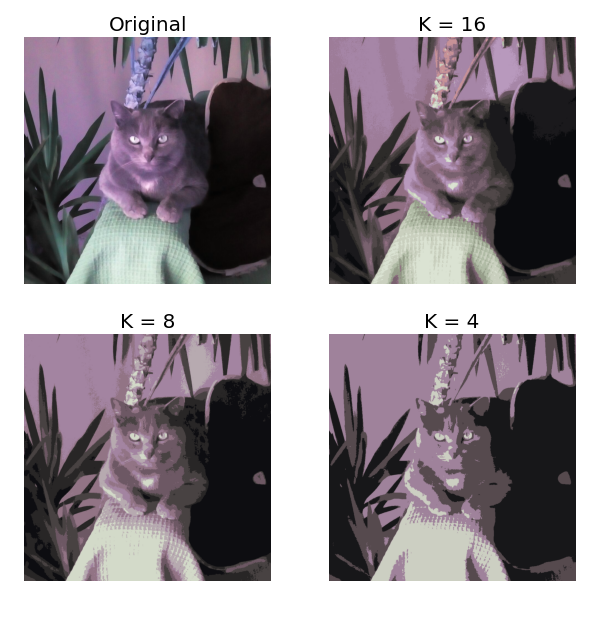
\includegraphics[scale=.3]{ColorQuantization.png}
		\caption{\textit{Color quantized GL image. We observe the original image, a 32 color image which look similar to the original one, a 16 colors image and 8 colors image. Tissue are grouped by color similarity. Reduce the color to the number of cluster allows pixel classification. }}\label{fig:ColorQuantization}
	\end{figure}

	Color quantization plays an important role in many application fields such as segmentation, compression, color texture analysis, watermarking, 
	text localization/detection, non photorealistic rendering and content-based retrieval~\cite{ART:Ozturk}.\\
	
	
	Color quantization is used for image segmentation. To this purpose the algorithm aim to reduce the number of colours in the image to the one of the different tissues,assigning a characteristic colour to each one of them. This is the case of medical image segmentation, in which each image color represents a particular characteristic of the tissue displayed (i.e in x-ray represent$\mu$). 
	To perform this technique, different algorithms may be used to group the colors, like clustering algorithm or the principal component analysis.


	
	
	
	

	
	
\end{document}
	\documentclass{standalone}
\begin{document}
		\subsection{U-Net}
		
		Artificial Neural Networks(ANN) are a computational architecture derived from neural physiological models~\cite{INP:Withey}. This architecture is made by interconnected artificial neurons able to perform elementary operations.  For imagery analysis are usually used Convolutional Neural Networks(CNN), also known as shift invariant or space invariant artificial neural networks (SIANN).\\
			
	
		In biological image processing 	the so called U-Net are usually used. U-Net is a kind of convolutional neural network which allows to overcome the requirement of many training data. That because large training dataset are not always available, like often happens in medical and biological segmentation purposes.
		
		Convolutional Networks are usually applied to classification tasks. In biological and medical purposes, the segmentation should include localization and a class label should be assigned on each voxel.
		To achieve this purposes, in $2015$ for the ISB cell tracking challenge, Olaf Ronneberger, Philipp Fischer, and Thomas Brox have developed this kind of network~\cite{ART:Johannes}.
		
		The U-Net is able to work with only small set of training samples. 	In order to work with few training data,we have to make a huge data augmentation, by applying an elastic deformation to the training images.
	
		The whole structure is divided into two main parts:
		\begin{itemize}
			\item Contraction path (\textit{encoder}) : sequence of convolutional and pooling layers, which aim
			to extract features and reduce the input dimensionality. 
			
			\item Expansion Path (\textit{decoder}) : second set of convolutional and up-sampling layers, to reconstruct the
			feature map and consequently the segmentation mask, which aims to process the extracted features
		\end{itemize}
	
		The contractive path and the extractive path. The contracting path is a typical convolutional network that consists of repeated application of convolutions, each followed by a rectified linear unit (ReLU) and a max pooling operation. During the contraction, the spatial information is reduced while feature information is increased. The expansive pathway combines the feature and spatial information through a sequence of up-convolutions and concatenations with high-resolution features from the contracting path~\cite{ART:Johannes}.
		
		Decode path tends to lose some of the higher level features that the encoder learned: Using shortcut connection, the output of the encoding layers are directly passed to the decoder layer, preserving the important features~\cite{PhDtheis}.
	
		
		\begin{figure}[h!]
			\centering
				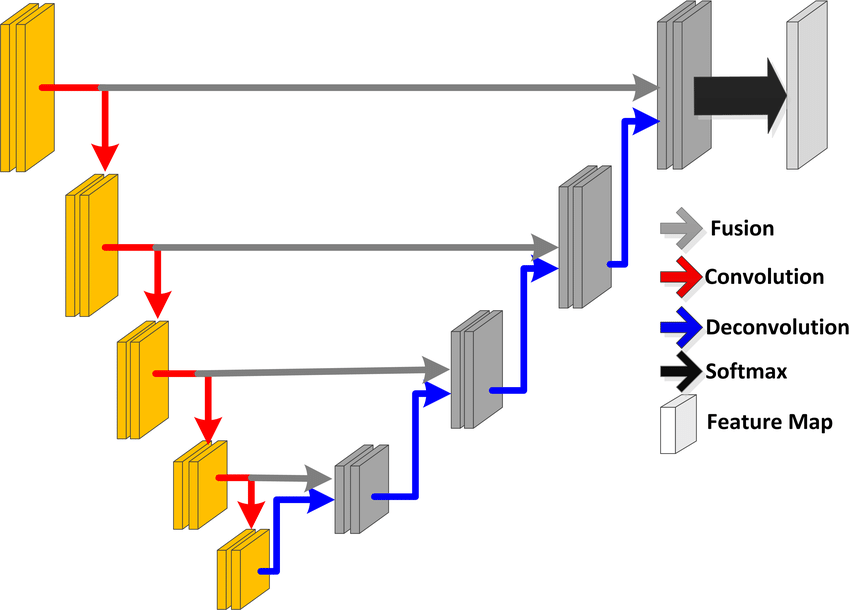
\includegraphics[scale=.4]{UNet.png}
					\caption{UNEt network architecture: We can see the U-shape made by symmetricity between expansion and contraction path. The gray arrows indicates the shortcut used to prevent information loss}\label{fig:UNet}
		\end{figure}
	
		
	
\end{document}MainSegmentation


	
\end{document}
\documentclass{standalone}
\begin{document}


	\documentclass{standalone}
\begin{document}
	\chapter{Results}

\end{document}
	
	%Pipeline description
	%\begin{document}
	
	\section{Pipeline}
	
	
	
	The aim of this works of thesis is to develop a pipeline for identification of GGO and CS areas in chest CT scans of patients affected by COVID-19, that aims to have the following characteristics:   
	\begin{itemize}
		\item  \textbf{Fully Automated: } to remove the dependency from an external operator, and so the subjectivity of the segmentation; 
		
		\item \textbf{Fast: } in order to compete with certified software and to provides a segmentation in few minutes.
	\end{itemize}

	Before going in deep and starting the description, I will define this kind of regions. 	
	Austin in ~\cite{ART:Austin} has defined the Ground Glass Opacities as an "\emph{Hazy increased attenuation of lung, but with preservation of bronchial and vascular margins; caused by partial filling of air spaces, interstitial thickening, partial collapse of alveoli,normal expiration, or increased capillary blood volume.}", which is different from consolidation in which bronchovascular margins are obscured. An example of these areas in displayed in \figurename\,\ref{fig:GGO}.

 %The whole pipeline was developed and tested on CT scans kindly provided by Sant'Orsola Hospital. Also the public datasets were used as benchmark. The used datasets are manually annotated; the provided labels are used to check the pipeline performances.\\ During the pipeline developing we have to takes into account that the infection regions may have different patterns according to the stage of the disease or recovery, as we can see in \figurename\,\ref{fig:GGO-Spatial}, and usually these patterns are spatially disconnected; so we have decided to use a pixel classification technique.\\
	
	
	\begin{figure}[h!]
		\centering
			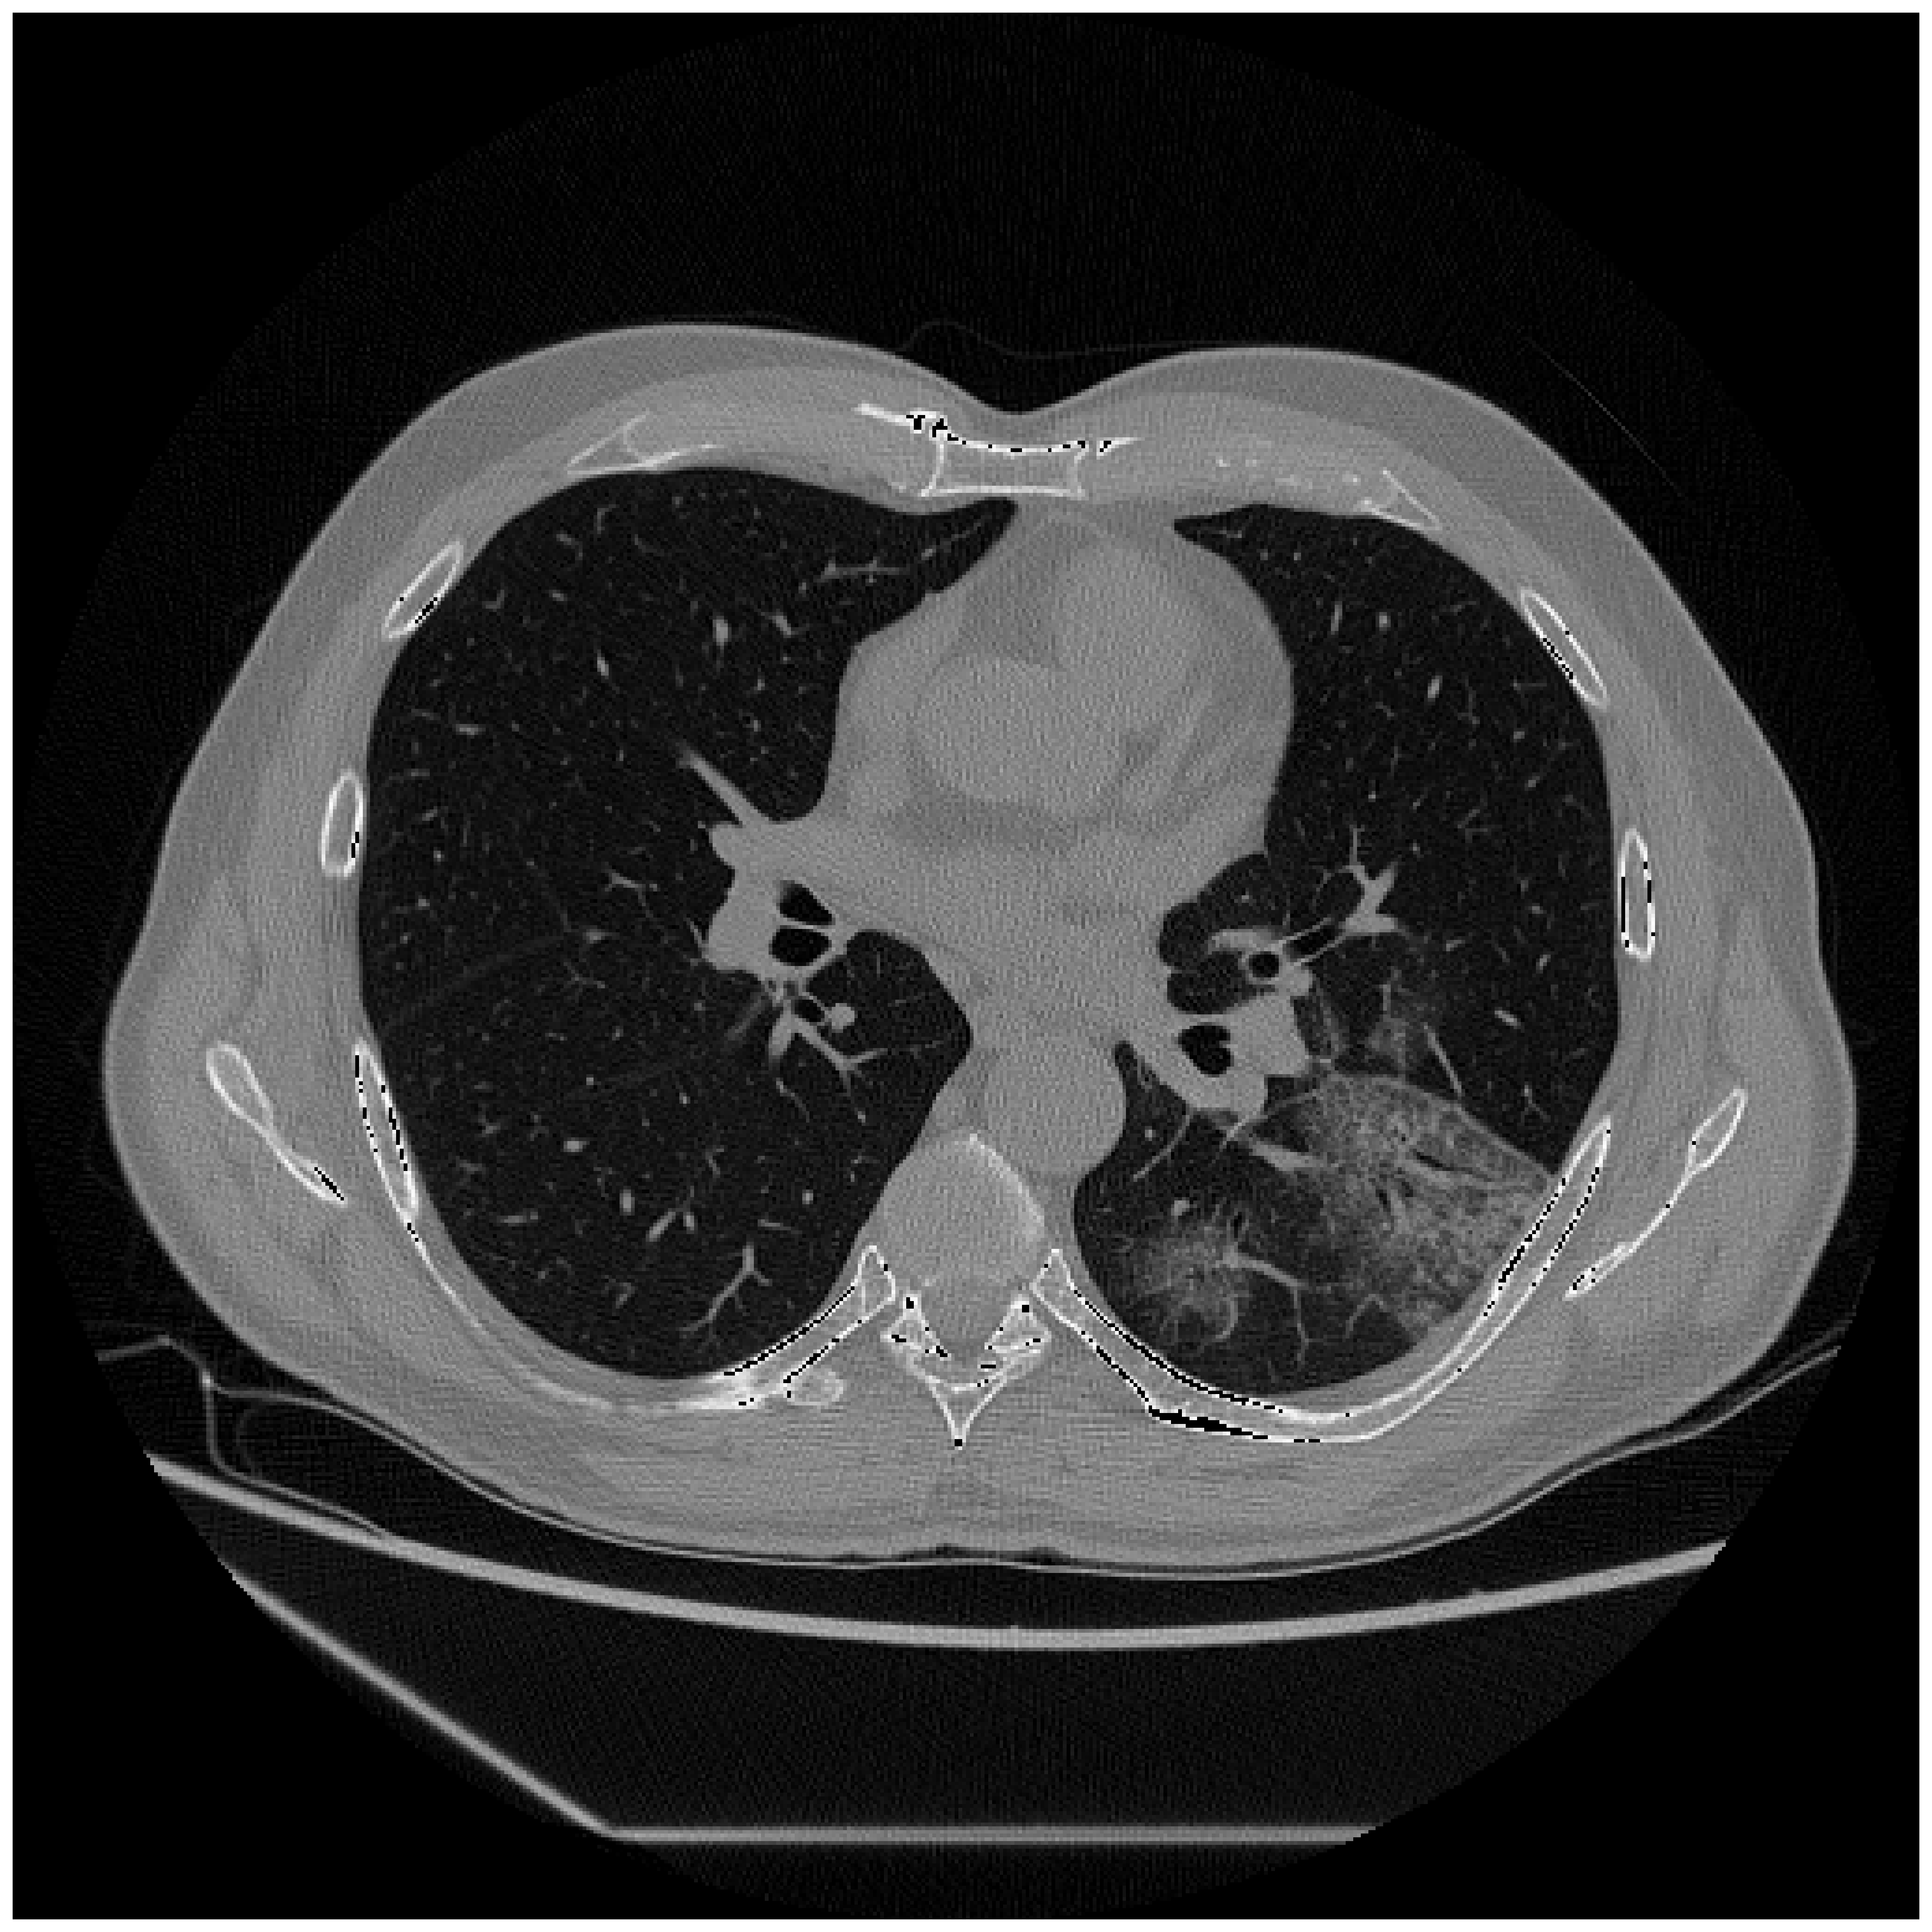
\includegraphics[scale=.5]{GGO.png}
		\caption{Chest CT image of a patient affected by COVID-19. We can see GGO and CS on the right lung. We can appreciate how the different structures, like lesions, are identified by similar color, so the basic segmentation idea was to group voxel by color similarity.}
	\label{fig:GGO}
	\end{figure}

	The segmentation is based on an unsupervised technique, so doesn't requires to provide the expected outcomes.
	As we can see in the chest CT scan in \figurename\,\ref{fig:GGO} the different structure are characterized by similar gray level: the basic idea was to use the color quantization for medical image segmentation, grouping voxel based on color similarity, and  assign  to each tissue a characteristic color. This can be done since in CT scan exist a relationship between the tissue in the voxel and the Gray Level used to display it, given by the Hounsfiend Units(eq\,\ref{eq:HU}), so colors are proportional to HU, which are defined as a linear transformation of the linear attenuation coefficient($\mu$).
		
	Color quantization and the properties of digital images allows to consider also other properties of the image besides the single voxel intensity:
	As I've said before, in digital image processing, images are represented with a 3D tensor, in which the first two dimensions represent the height and width of the image  and the last one the number of channels. 
	In this work we have used the different channels to takes in account different properties, exploited by the application of suitable filters on the original scan. This allow us to consider also neighboring voxels, that is really suitable for the segmentation since the  lesions areas involves many closest voxels, not only a single one. 
	
	Once we have build the color space, we have to found the characteristic color of each tissue under study, which is represented by a centroids in the color space. In order to perform this task and achieve the centroids estimation, a simple k-means clustering was used, since it provides a suitable segmentation with good time performances and it is efficiently implemented for multi-channel images in \textsf{OpenCV}~\cite{OpenCV}.
	 
	K-means clustering requires a prior knowledge about the number of cluster, which in our case is given by the anatomical structure of the lung; so we can consider a different cluster for each anatomical structure.
	Once we have estimated the centroids for each tissue, we have used them for the actual segmentation, by assign each voxel to the cluster of the closest centroids: in this way the estimation step, that we will call "train", needs to be performed only once, so can be time expansive since is not involved in the actual segmentation.\\
	
\end{document}
	\documentclass{standalone}
\begin{document}
	\subsection{Pipeline Structure}
	
	In this section I will discuss the general structure of the pipeline, more details about the actual implementation will be given in the next chapter.
	To perform the color quantization I've to found the characteristic color(centroids in the color space) of each tissue and use them for the actual segmentation, dividing the pipeline in two main steps. Before each of these steps we need a preliminary phase that aim to isolate the lung regions in order to exclude the extra lung areas and reduce the false positives and motion artifacts.
	In the end the pipeline structure is divided in three main blocks as we can see in \figurename\,\ref{fig:Pipeline} : 
	\begin{itemize}
		\item \textbf{Pre-Processing and lung extraction}: Preliminary step, involves registration of HU, isolation of lung regions and removal of bronchial structures and air pockets.
		
		\item \textbf{Training} : estimation of the centroids, is performed only ones; 
		
		\item \textbf{Labeling} :  assignment of each voxel to the cluster of the closest centroids, it is the actual segmentation.
	\end{itemize}
	
		
	\begin{figure}[h!]
		\centering 
			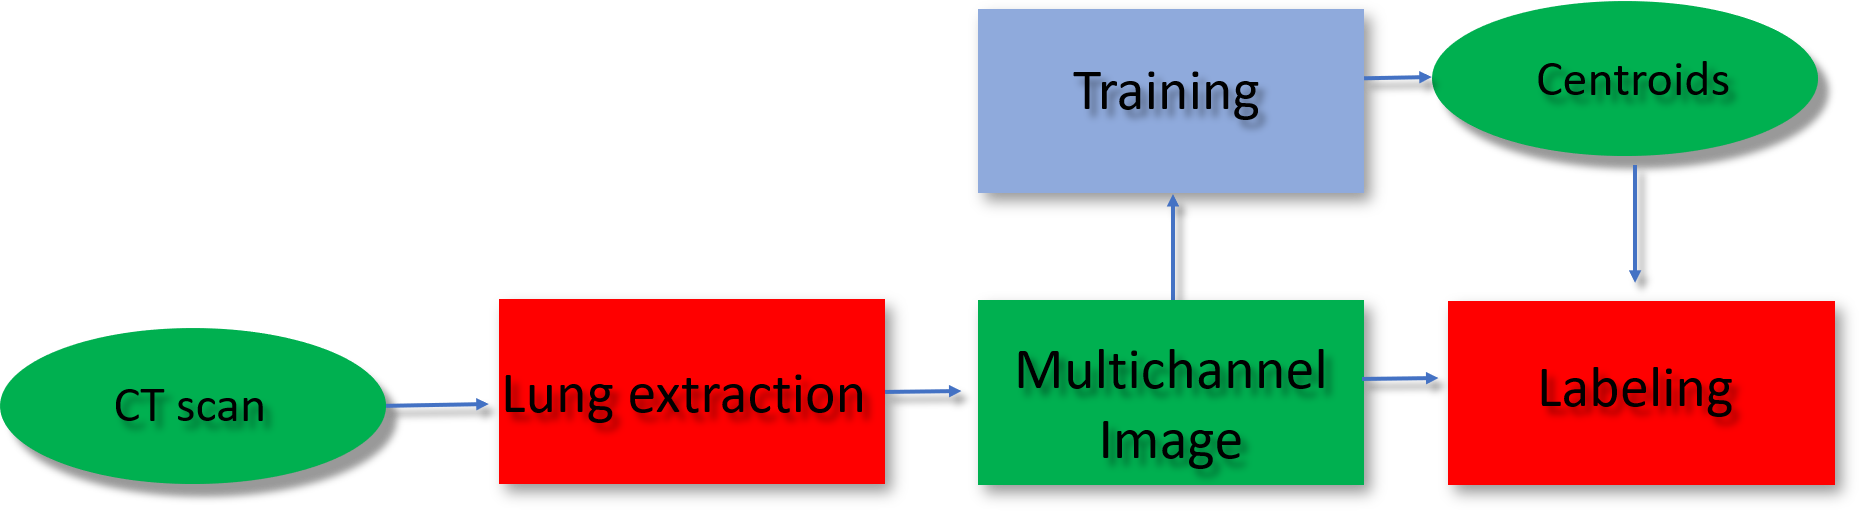
\includegraphics[scale=.65]{Pipeline.png}
		\caption{Flow chart of the main structure of the developed pipeline. The training process, which allows the estimation of the centroids, is performed only one time.}\label{fig:Pipeline}
	\end{figure} 
	
	\subsubsection*{Pre Processing and Lung Extraction}
	
	This preliminary step is performed before both training and labeling; involves the managing of the HU, the isolation of lung regions and the removal of the bronchial structures.\\
	The registration of the HU on a common space in necessary to overcome the issues that may raise from the different padding values and multiplicative constant for HU computation(equation\,\ref{eq:HU}) used by the different manufacturer of the CT scans.\\
	Lung segmentation is pivotal pre-processing step in many image analysis such as classification, identification and classification of lung pathologies~\cite{ART:Johannes}. The lung isolation allow us to found a mask for the lung regions, excluding so all the body regions, the CT tube and the extra-lung organs like intestine and heart, avoiding the fomation of false positives.\\
	Automatic lung segmentation algorithm are typically developed and tested on limited dataset and usually over a limited spectrum of visual variability by containing mainly cases without severe pathologies~\cite{ART:Johannes}. Rule based approach, like thrasholding, region growing, ect, usually fails for CT sans of patients with severe ILD, as we can see in \figurename\,\ref{fig:UNetVSThr}. So, to achieve the lung segmentation I've used  pre-trained UNet~\cite{ART:Johannes}~\cite{REP:lungmask}, that provide a good segmentation of the lung regions. 
	The UNet is a supervised approach, however is used only on this preliminary step, as we will see the identification of infection regions is made with an unsupervised approach.\\
	
	\begin{figure}[h!]
		\centering
		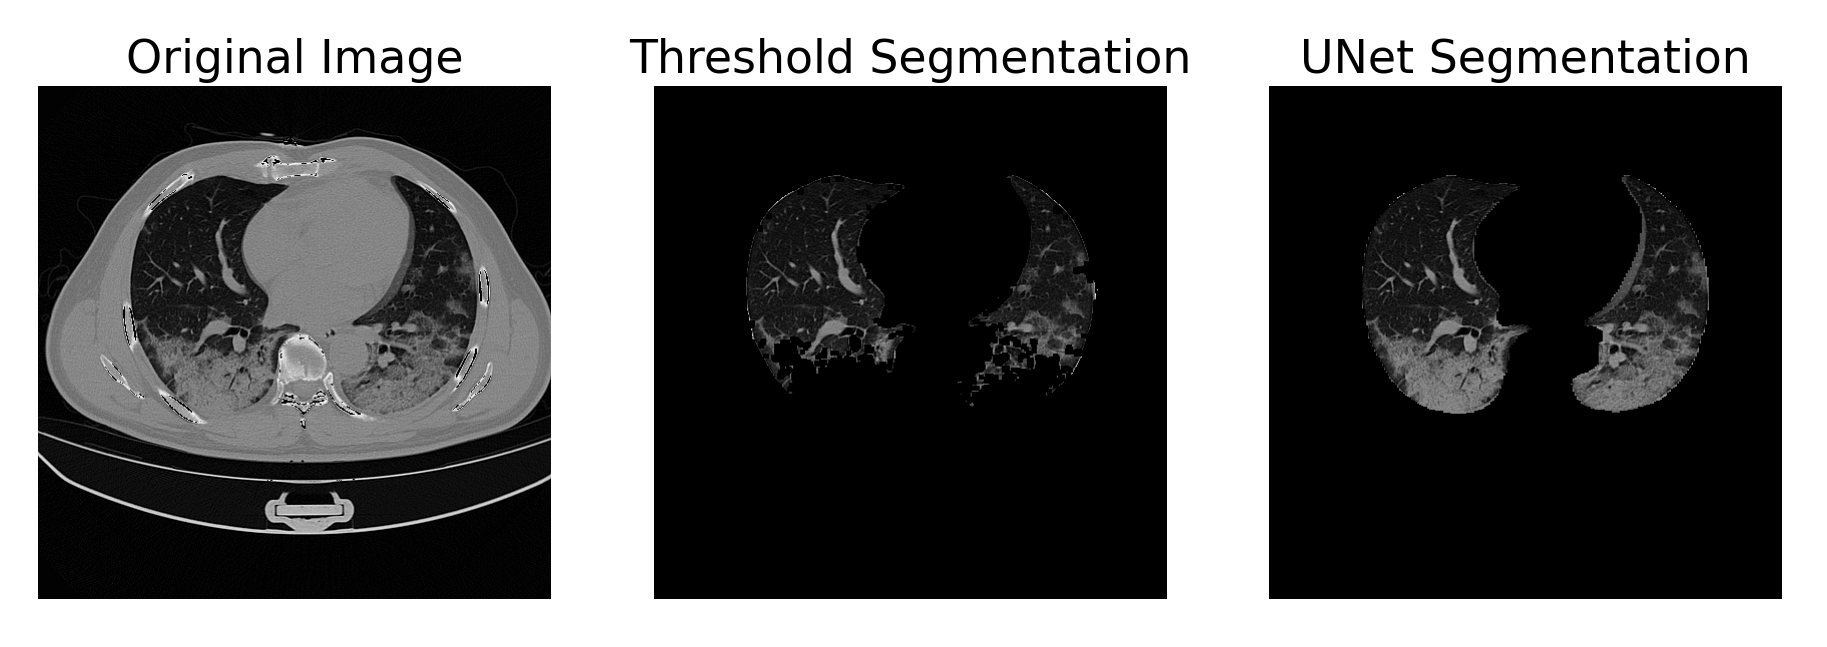
\includegraphics[scale=.5]{UNetVSThr.png}
		\caption{From left to right the original CT scan of a patient with severe ILD, the lung segmented by threshold and connected components, UNet lung segmentation. We can clearly see the missing areas in the fist segmentation, corrected identified in the UNet one.}\label{fig:UNetVSThr}
		
	\end{figure}
	
	This kind of segmentation include in the lung region also motion artifacts and air-pockets, which we will see are the principal cause of false positives. To achieve a better segmentation a refinement process is performed, which aims to remove the main bronchial structures form the selected lung regions. Up to now no motion artifact removal routines is implemented, so we will see that this kind of artifacts wil be the main source of misclassified points. 
	
	\subsubsection*{Training}
	
	This step involves the estimation of the centroids for each tissue. To achieve this purpose we have chose to perform a clustering by using the k-means algorithm. We have to takes into account that the k-means clustering requires an homogeneous representation for each cluster. As we will see we have to manage this problem. Moreover the patient that have a low involvement of lung parenchima have the cluster corresponding to the infection underrepresented, to overcome this issue a careful selection of the patient used for the training was performed. 
	In summary, the implementation of this step involve the building of the multi-channel image, which allow us to takes into account also the neighbouring information, the managing of the over represented clusters  and the actual centroids estimation.

	\subsection*{Labeling}
	
	This step involves the actual segmentation. The script which perform it requires as inputs the CT scans after the lung extraction, and the previously estimated centroids. This block of the pipeline simply assign each voxel to the cluster corresponding to the nearest centroids and the select only the one corresponding to GGO and CS. In this way we are performing a pixel classification by assign regions to a particular labels according only to intensities information, without exploiting spatial information: this allow us to group on the same cluster objects that are spatially disconnected as often happen in medical imaging field.\\
	The distance between voxel color and each centroid is defined as euclidean distance:
	\begin{equation*}
		d(x_j, c_i) = \sqrt{(x_j - c_i)^2}
	\end{equation*} 
	Where $x_j$ is the color vector for the $jth$ voxel and $c_i$ is the $ith$ centroid.\\
	
	To summarize, once the centroids are estimated, the segmentation pipeline will results in $2$ main steps : \textbf{lung extraction} and \textbf{labeling}, as shown in \figurename\,\ref{fig:FinalPipeline} in which we can observe the flowchart of each step with an image that shown the partial results.
	
	\begin{figure}
		\centering
			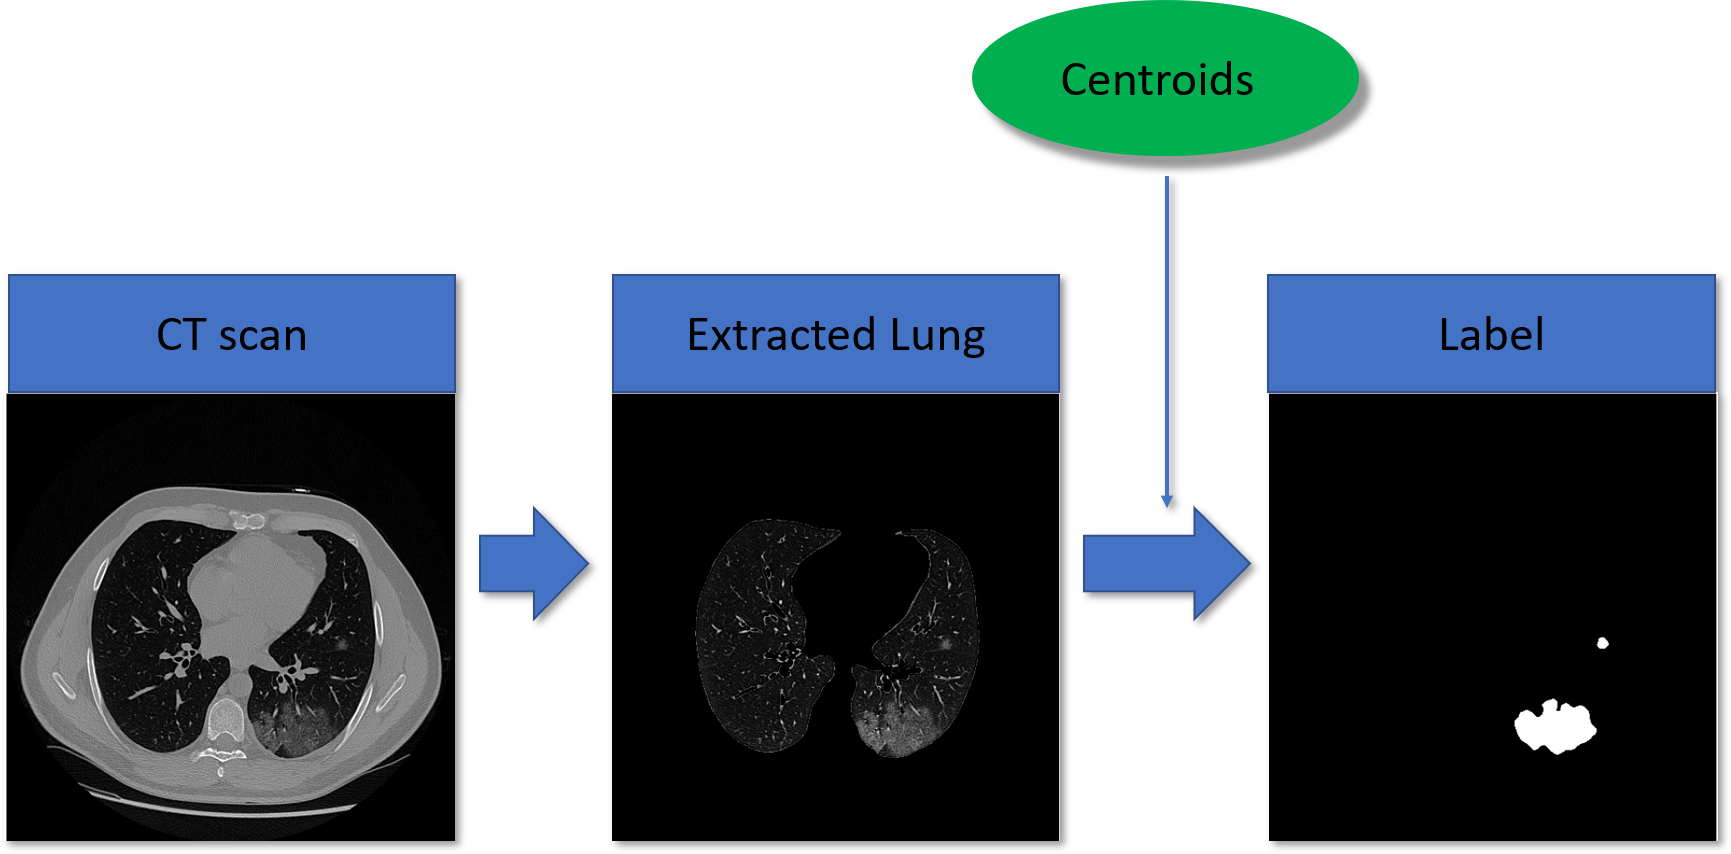
\includegraphics[width=.87\textwidth]{final_pipeline.png}
			\caption{Actual segmentation step, from left to right we can see the input image stack, the isolated lung regions and the final label. To performed the labeling a set of pre-computed centroids was used.}\label{fig:FinalPipeline}
	\end{figure}
	
	
	
\end{document}
	
	% pipeline implementation 
	\begin{document}
	
	\section{Pipeline Implementation}
	
	
	In this chapter I will describe in details the actual pipeline implementation. First of all I will briefly describe the used framework for the actual implementation. After that I will describe step by step each block of the pipeline, describing how each task is achieved.\\
	
	The whole pipeline was implemented by using python, which is an high level object oriented programming language and to perform the necessary image processing operations, the managing of input and output images, and the other operation I've mainly used OpenCV~\cite{OpenCV} and SimpleITK; for the other operations involving the image tensor I've used Numpy~\cite{Numpy}\\
	Since python is an high level language, it allows an easy and fast implementation of the code, on the other hand working with optimized image processing libraries written in C++ allows to prevent the lack of performances.\\
	
	The whole code is open source and available on github~\cite{REP:CTLungSeg} and the pipeline installation is automatically tested on both Windows and Linux by using AppveyorCI and TravisCI.  The installation is managed by setup.py, which provides also the full list of dependencies. The code documentation was generated by using sphinx and its available at \url{https://covid-19-ggo-segmentation.readthedocs.io/en/latest/?badge=latest} . To automatize the segmentation on multiple CT scans are provided bash and powershell script and,  even if the centroids are already estimated, a training script is provided, in order to allow the user to estimate its own set.
	
	The whole pipeline is organized into three scripts, which performs the main tasks: 
	\begin{itemize}
		\item lung\_extraction
		\item train
		\item labeling
	\end{itemize}
	
	The usage of SimpleITK to manage input and output file, allows the compatibility with medical image formats and the preservation of the spatial information.
\end{document} 

	%\documentclass{standalone}
\begin{document}
	
	\subsection{Frameworks}
	
	In order to perform all the necessary image processing operations both involving 2D and 3D filters, to perform the color quantization and to manage the input and output medical image format, I've used mainly two libraries for image processing and computer vision. These libraries has been written in C++ but has multi language support. I've performed all the 2D image processing operations like median blurring or filter application by using \textsc{OpenCV}~\cite{OpenCV}. For the managing of medical image formats, ensuring the preservation of voxel spatial information, and for the 3D operations, I've used \textsc{SimpleITK}.  To perform all the other operation on the image array, I've used \textsc{Numpy}~\cite{Numpy}.
	
	For the preliminary lung extraction, I've used the pre trained Unet available on GitHub(\url{https://github.com/JoHof/lungmask}).
	
	\subsubsection*{OpenCV} 
	
	\textsc{OpenCV}, acronym for Open Source Computer Vision, is an open source computer vision and machine learning software library. \textsc{OpenCV} was built to provide a common infrastructure for computer vision applications and to accelerate the use of machine perception in the commercial products. This library is implemented in C++, however bindings are available for \textsc{Python}, \textsc{Java} and \textsc{MATLAB/OCTAVE}. This library can use also hardware acceleration like Integrated Performance Primitives, and also  \textsc{CUDA} and  \textsc{OpenGL} based  \textsc{GPU} interfaces are available. 
	
	I've used the tolls from this library to perform all the processing that involves the single image and, most important, to perform the color quantization, since the k-means implementation offered by the library allows to cluster multi channel images in an efficient way.
	
	\subsubsection*{SimpleITK} 
	
	\textsc{SimpleITK} is a simplified programming interface to the algorithms and data structures of the Insight Toolkit ( \textsc{ITK}) that support many programming languages. The library provides a simplified interface to use Insight Tool Kit(ITK) library. 
	Insight Tool Kit (ITK) is an open source library which provides an extensive suite of tools for image analysis, developed since 1999 by US National Library of Medicine of the National Institutes of Health.This library provides tool useful to works also with N-dimensional images. 
	This library provides a powerful tools for the reading and writing of the image. Since \textsc{ITK}, ans so \textsc{SimpleITK},  consider the image like spatial object and not like arrays of values, it store also information about voxel spacing, size and origins, provided as well as the array, this makes us able to works only with the array by using \textsc{Numpy} or \textsc{OpenCV}, by preserving the spatial information of the image.
	
	\subsubsection*{Numpy}
	
	\textsc{Numpy} is an open source project aiming to enable numerical computing with Python. It was created in 2005, building on the early work of the Numerical and Numarray libraries.	\textsc{Numpy} is developed in the open on GitHub, through the consensus of the \textsc{Numpy} and wider scientific Python community.~\cite{Numpy}. \textsc{Numpy} allows to works with large $n-$dimensional tensors., together with a large set of functions to operates with them.\\
	This libraries was used to operate to the CT scan tensor. 

	\subsubsection*{Pre-Trained UNet} 
	
	This network is a pre trained UNet which allows an Automated lung segmentation in CT under presence of severe pathologies. The whole code is written in python and it is based on torch and torchvision libraries. The repository offers 4 pre trained models for different kind of segmentation, like single lung lobe segmentation and the extraction of lung in presence of severe ILD. Each model perform the segmentation slice by slice. 
	
	The used network is a U-Net,that is a modification of the convolutional neural network architecture useful for medical and biological field, because is developed to works also with a small training dataset.
	The allowed pre-trained models are the follows : 
	\begin{itemize}
		\item \textbf{R231} : This model, trained on a dataset that cover a wide range of visual variability, performs a segmentation on individual slice and extract the right and left lung lobes including airpockets, tumor and effusion, wothout including the trachea.
		
		\item \textbf{LTRCLobes} : This model, trained on a subset of LTRC dataset, perform an individual segmentation fo lung lobes, but have limitad performances in case of severe ILD.
		
		\item \textbf{LTRCLobes\_R231} : Model which fuse the two previous one. Fills the false negative of LTCTLobes by using R231, but is computational expansive.
		
		\item \textbf{COVID231-Web} : Augmentation of R231 with COVID-19 slices that were mapped back from regular imaging formats to HU The data was collected and prepared by MedSeg. 
	\end{itemize}
		
	
	The network was trained in order to takes the maximum flexibility with respect of the field of view, in order to enable the segmentation without a prior localization of the organs.
	
	The model is trained on $231$ CT scans collected from PACS, selected following these criteria: 
	\begin{itemize}
		\item Random Sampling ($57$ scans)
		
		\item Sampling from Image Phenotypes (71 scans)
		
		\item Manual selection of edge cases : 
			\begin{itemize}
				\item Fibrosis ($28$ scans)
				
				\item Trauma ($20$ scans)
				
				\item Other Pathology ($55$)
				
			\end{itemize}
	\end{itemize}

	That ensure a proper variability of the training dataset.
	
	 The \textbf{COVID231-Web} was used developed to incorporates collections of slices and case reports from the web are often cropped, annotated or encoded in regular image formats so that the original hounsfield unit (HU) values can only be estimated.  Since the scans used in this works do not fall within these cases, we have used the the \textbf{R231} model, which works very well with COVID-19 CT.
	
	 
\end{document}
	\documentclass{standalone}
\begin{document}
	\subsection{Lung Extraction}
	
	This script aims to achieve the HU registration, the lung segmentation and the bronchial removal. It takes as input the CT scan in each format supported by \textsc{SimpleITK}. As output will returns the stack after the lung extraction in \textit{nifti} format. Also other medical image format are supported. Its workflow is summarized in\ref{alg:lungExtraction}.
	
		 
	\begin{algorithm}
		
		\SetAlgoLined
		\DontPrintSemicolon
	
		\KwData{Volume (CT scan)}
		\KwResult{Volume with extracted lung}\;
		
		mask$\leftarrow$ApplyUNetVolume(Volume)\;
		
		volume$\leftarrow$(volume < 1200) =air\_hu\;
		volume$\leftarrow$ShiftMinimumTo1(volume)\;
		
		\tcc{Start the bronchial removal}\;
		
		eigen$\leftarrow$ maxEigenvalues(lung)\;
		bronchial\_mask$\leftarrow$ (eigen < threshold)\;
		lung\_woBronchi$\leftarrow$ (lung $\circ$ bronchial\_mask)\;
		
		\tcc{Refine the bronchial mask}\;
		
		eigen$\leftarrow$maxEigenvalues(lung\_woBronchi)\;
		bronchial\_mask$\leftarrow$(eigen < threshold)\;
		lung\_woBronchi$\leftarrow$ (lung\_woBronchi $\circ$ bronchial\_mask)\;
	
		\caption{Lung Extraction}\label{alg:lungExtraction}
		
	\end{algorithm}
	
	
	The lung mask was created by applying the suitable method from~\cite{REP:lungmask}. 

	In order to achieve the first step, first of all all the values less than the air value are setted to this value, after that the air value is subtracted from all the voxels. These operation are performed on the image tensor by using \textsc{Numpy} ndarray method.  
	
	\lstset{style=python}
	\begin{lstlisting}[language=python, caption=HU registering function, label=code:saf]
		
	import numpy as np
		
	def shif_and_crop(tensor) :
		
		tensor[tensor <  -1200] = tenor[tensor > -1200].min()
		tensor = tensor - tensor.min()
	
		return tensor
	\end{lstlisting}

	More inreresting is the estimation of the eignevalues map. To achieve this purpose I've implemented a function based on \textsc{cv2.cornerEigenValsAndVec} in \textsc{OpenCV}. This function takes as input an $8-$bit gray scale image, so we have to rescale the GL value of the obtained image tensor. Since I don't want to lose information about the rescaled values, I've simply made a copy of this object. 
	
	In the end the computing of the eigenvalues map is made by the following function: 
		\lstset{style=python}
	\begin{lstlisting}[language=python, caption=HU registration function, label=code:saf]
		
	import cv2
	import numpy as np
	from functools import patial
		
	def max_eigenvalues_map(tensor, block_size, kernel_size) :
		
		func = partial(cv2.cornerEigenValsAndVecs, 
						blockSize = block_size, 
							ksize = kernel_size)
		res = np.array(list(zip(*list(map(func, tensor)))))
		res = res.transpose(1, 0, 2, 3)
		res = res[:, :, :, :2]
		max_eigenvals = np.max(res, axis = 3)
	
		return max_eigenvals

	\end{lstlisting}

	Once the required parameter were setted, the \textsc{OpenCV} function is iterate over the axial slices. The following transposition and selection of tensor elements, are needed since the function returns also the eigenvectors, in which we are not interested in. 
	
	At the end of the whole procedure, the resulting tensor is saved into a medical image formats. 
	%This is a pre-processing step, which involves the creation of a lung mask and the managing of the Hounsfield Unit. The creation of a mask for the lung regions aims to reduce the number of clusters and avoid the formation of false positives by removing external structures, which can be source of errors. In order to achieve this purpose, I have decided to use a pre-trained neural networks~\cite{REP:lungmask} which code is open source. 
	
	%\textbf{red}{Once we have found a suitable mask for the lung, a managing of HU must be performed. The $k$ constant in the HU definition (equation\,\ref{eq:HU}) may change according to the scan manufacturer or scan model; moreover, during the scan acquisition, all the regions outside the CT tube aren't sampled, so to obtain a square $N\times N$ image for each slice some padding values are added, which different values according to the scan manufacturer: for instance in the CT scan in \figurename\,\ref{fig:Pre-Processing}(a) the padding value is $-3000 HU$ and the air value is $-1024$. }
	
	%The first thing to do is to make the padding value and the air value equal for each scan considered and shift them to $1$: in this way we have registered the HU for scan from different manufactures in a common space, as we can see in \figurename\,\ref{fig:Pre-Processing}(b).
	
	 %May happen that some patients have metallic prothesis, so metallic artifact may be present. Since usually this implant are outside the lung, are removed after the mask application, so no other step are needed.
	 
		%\begin{figure}[h!]
		%\centering
		%%\subfigure[Histogram of a CT scan before registration]
	%	{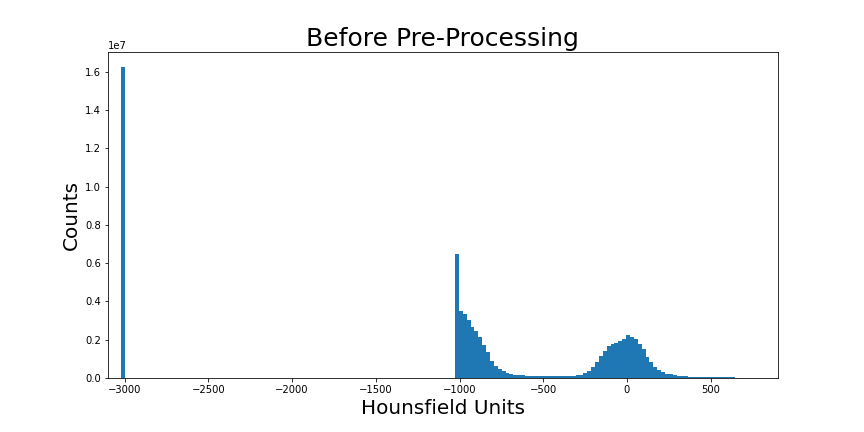
\includegraphics[scale=.3]{HU_before_rescaling.png}}
	%	%\hspace{1mm}
	%	\subfigure[Histogram of a CT scan after the registration]
	%	{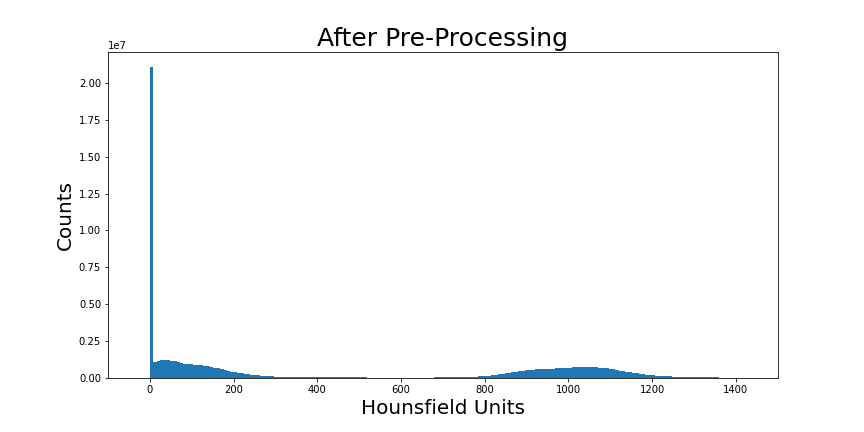
\includegraphics[scale=.3]{HU_after_rescaling.png}}
	%	\caption{Histogram of voxel values before and after the pre-processing. We can observe that before the pre processing there are some HU out of range, which are the values used to fill the regions outside the tube, and the air value is around $-1000\,HU$ according to HU definition. After the rescaling we can observe that all the values are non-negatives.}\label{fig:Pre-Processing}
	%\end{figure}
	%Now, we have found the mask for the lung regions, and we have managed the HU, so by a simple element wise AND we are able to isolate the lung from the rest of the body, removing also the organs, like heart and intestine, presents in the CT scans.
	
	%We have observed that the presence of the bronchial structure in the lung regions is one of the main source of false positives, so an extra step was added in order to remove as much as possible this kind of structures.
	
	 %Bronchi have an elongated shape respect to the other structure which usually are rounded: the basic Idea was to use this kind of information, by using the \href{https://www.docs.opencv.org/master/dd/d1a/group__imgproc__feature.html#ga04723e007ed888ddf11d9ba04e2232de}{cornerEigenValsAndVecs} function implemented in \textsc{OpenCV}. This particular filter compute the covariant matrix of the derivative in a neighborhood and the corresponding eigenvalues. If a particular regions has an elongated shape, one of the eigenvalues (corresponding to the eigenvector in the direction of the structure) will have an higher value, otherwise both eigenvalues have a lower value. So we have applied this filter on each slice of the scans and took the maximum eigenvalues. 
	%\begin{figure}[h!]
	%	\centering
	%		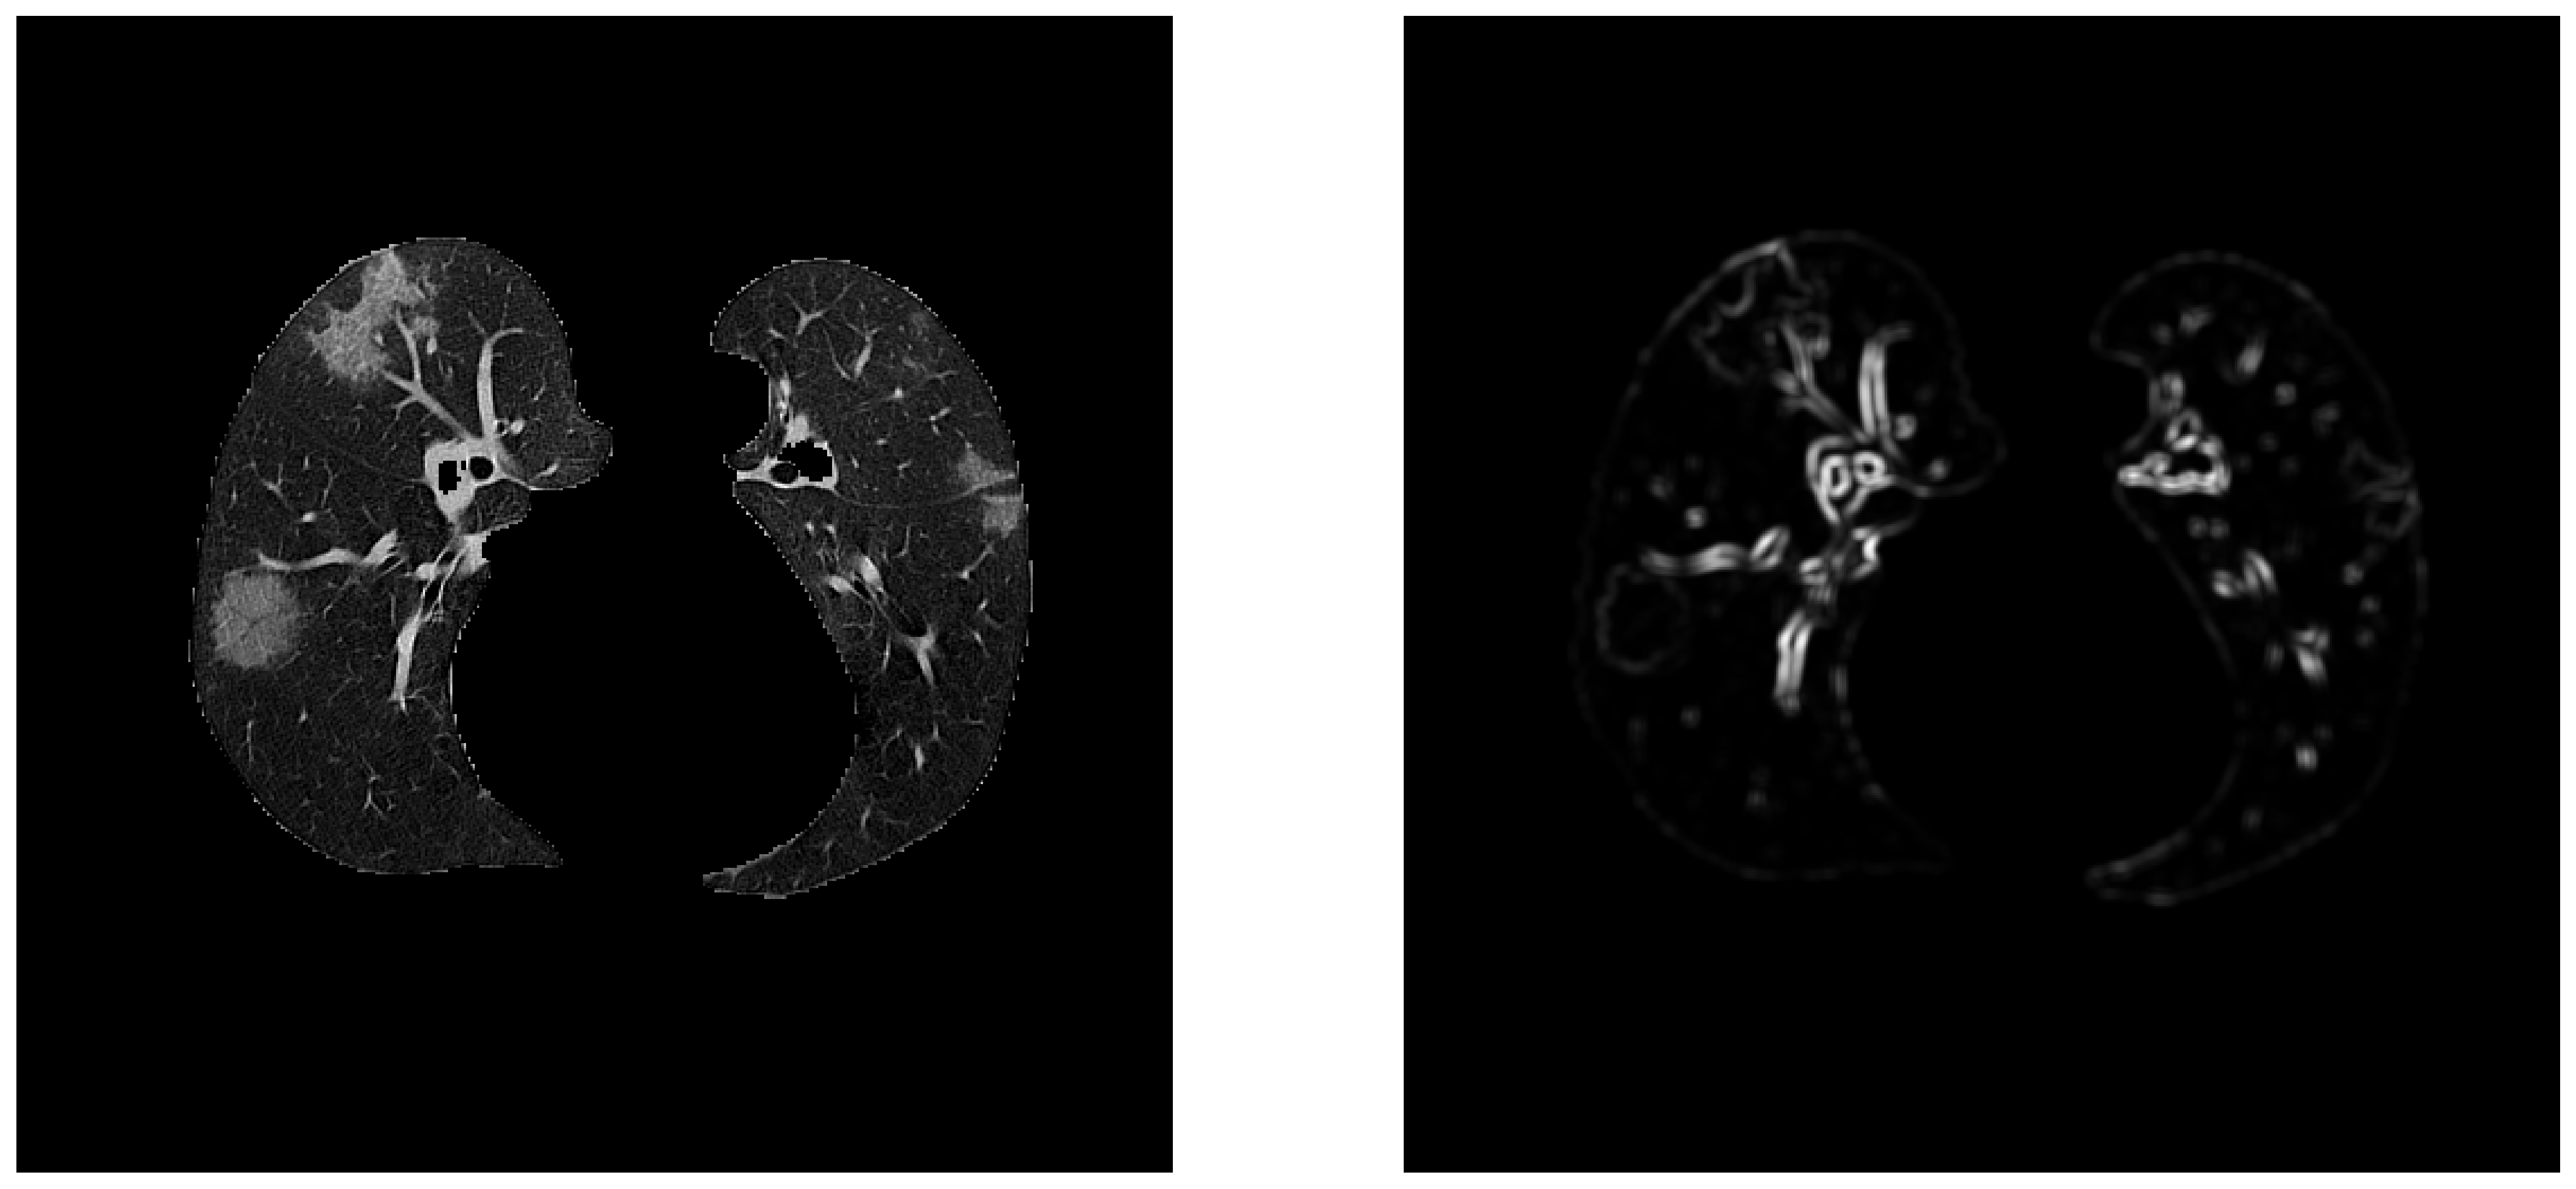
\includegraphics[scale=.3]{MaxEigenVal.png}
	%		\caption{From left to right: lung regions selected by the U-Net; ,maximum eigenvalues map of the lung. As we can see the U-Net does not exclude the bronchial structure from the lung, on the other hand, the maximum eigenvalues map delineates very well these regions.We have used this map to remove the unwanted bronchial regions.}\label{fig:MaxEigenval}
	%\end{figure}

	%In \figurename\,\ref{fig:MaxEigenval}, I've displayed the image after the lung segmentation by the neural network, and the corresponding eigenvalues map. As we can see the higher values of the map corresponds to the edges of the main bronchial structures. To create the mask for these structures a simple threshold on the map was taken. Since the main bronchial structures are large, this process is able to remove only part of the edges, but the inner structure is preserved. In order to refine the segmentation, this process is repeated a second time, allowing a more accurate exclusion of the structures.
			
\end{document}
	\begin{document}
	
	\subsection{Training}
	
	This step consist in the estimation of the centroids of the color space. May be  really time consuming, but it is performed only once, so during the actual segmentation the corresponding script isn't run.\\
	To achieved the estimation of centroids, a k-means clustering of the multichannel images of several CT scan from different patients is performed. 
	In order to achieve a uniform representation of each cluster, the scans included in the training set were carefully selected from the $3$ datasets used in this work. The main rule used for the selection is that in each scan must me present a huge amount of infection areas and also a well representation of artifacts, in order to takes into account all the possible features.\\
	The achievement of this task involves two main steps : 
	\begin{enumerate}
		\item \textbf{Preparation of images} : involves the building of the multi channel images, and the registration in a common space; 
		
		\item \textbf{Clustering} : Actual clustering, involves also the managing of the background problem.
	\end{enumerate}

		\subsubsection*{Preparation of Images} 
	
		This step involves the preparation of images, with the building of the multi channel image that incorporates neighbouring and edges information as well as the registration in a common space and the managing of an allocation memory problem.\\
			
		As I've said the multichannel image is build to incorporate more information during the clustering. We have found that a 4 channel image will provides good segmentation results. The 4 channel of the image are built as follows  : 
		\begin{itemize}
			\item Pure image after histogram equalization; 
			\item Median Blurring of the equalized image; 
			\item Gamma corrected image;
			\item Standard filtered image.
		\end{itemize}
	
		\begin{figure}[h]
			\centering
				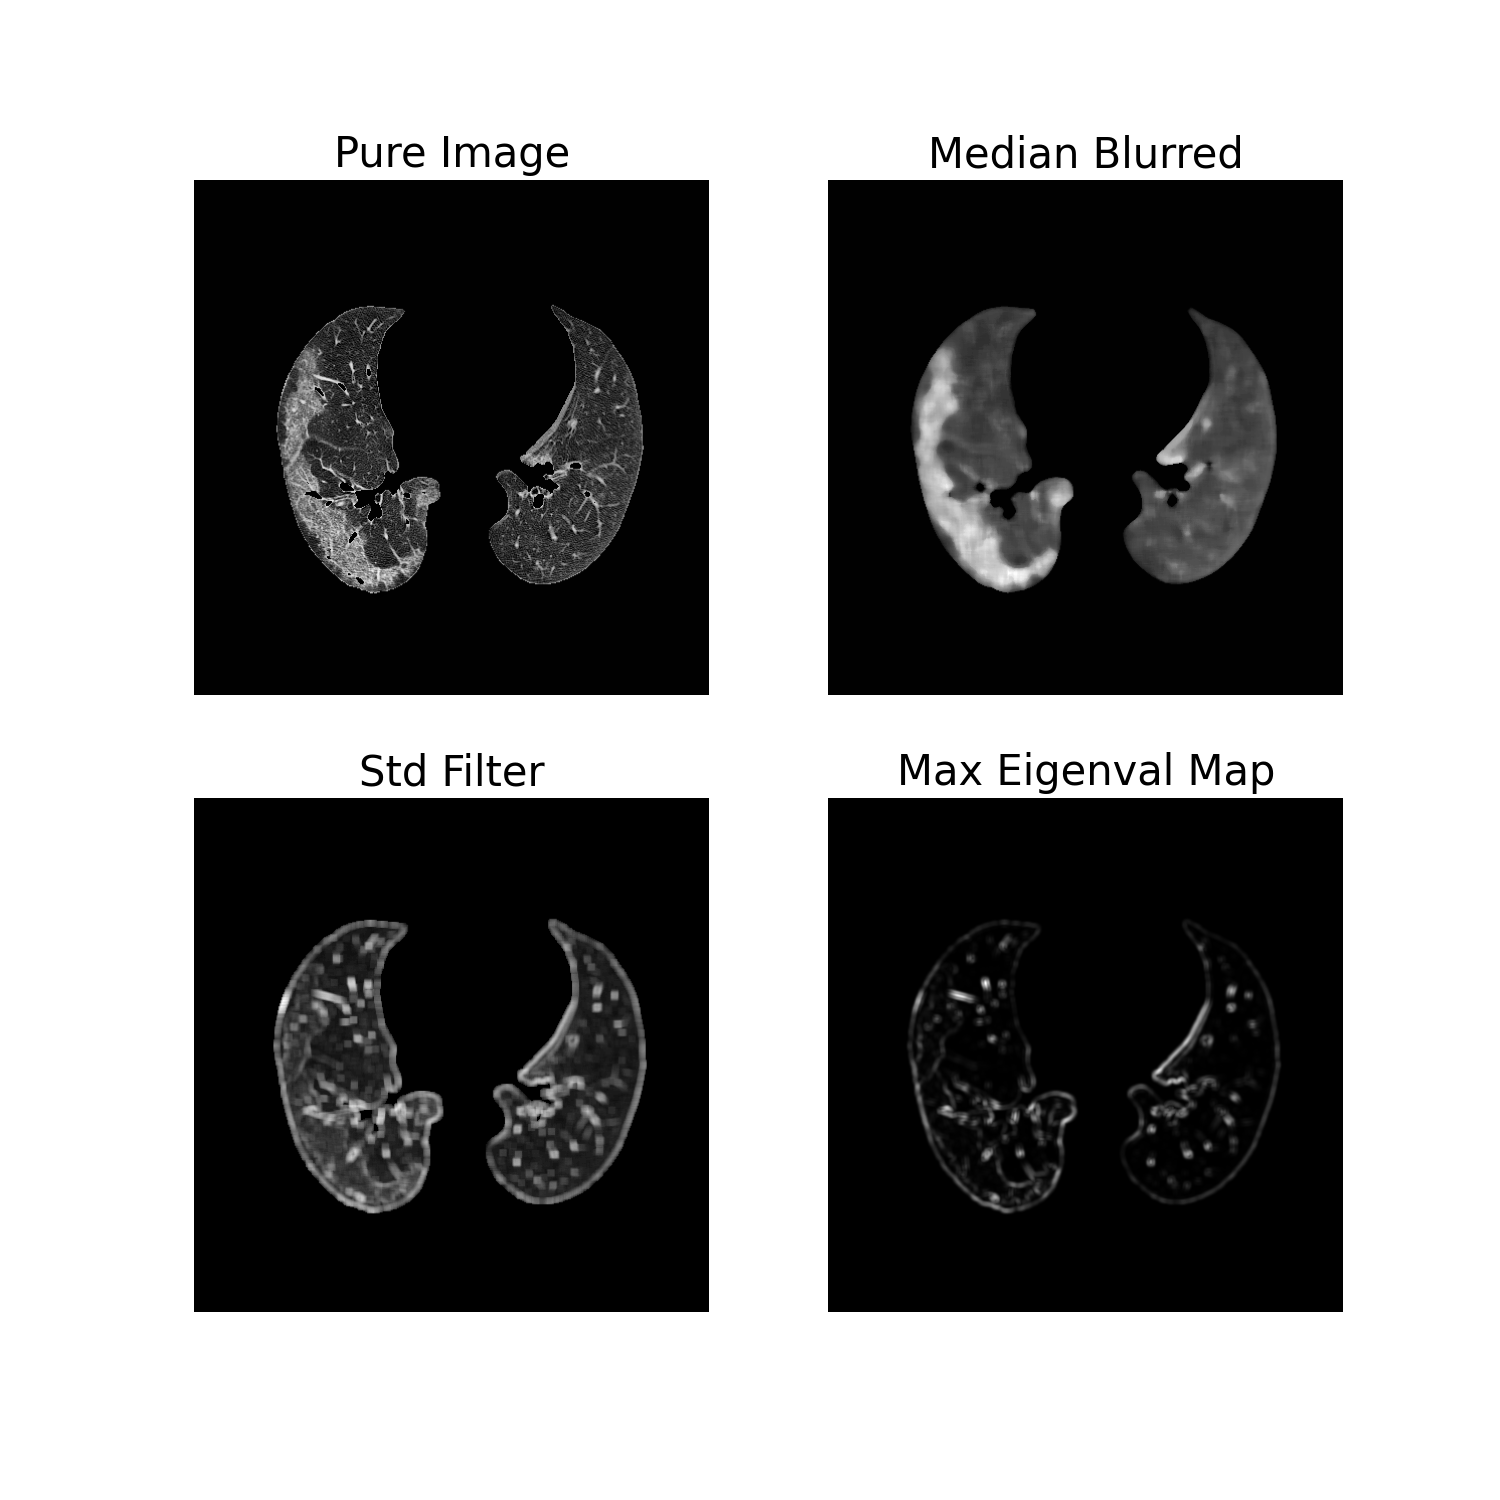
\includegraphics[scale=.55]{Multi_Channel.png}
			\caption{Channels of the image. From left to right and from top to bottom the imageaffter the histogram equalization, the gamma corrected image, the median blurred image and the std fitered image. This channels allow us to consider informations about the single voxel but also about the neighbouring voxels and their variability. }\label{fig:MultiChannel}
		\end{figure}
	
		In \figurename\,\ref{fig:MultiChannel} I've displayed the 4 different channel of the image. Each channel allow us to consider different information\\
		The histogram equalized image and the gamma corrected allows to takes into account information about the single voxel. The histogram equalization is applied in order to ehance the image contrast by improving the GL usage. For each slice the histogram is equalized operatiing in small image regions, in order to takes care of the over-amplification of the contrast.\\ The gamma correction is a non linear operation and is used to decode the lumnance, and to made in evidence the less evident lesions. Both of this filters involves the single voxel.\\The median blurring allow us to consider also the information of the neighborhood voxels, allowing the reduction of the outliers. The usage of this filter is justified since the lesions involves several closest voxels.\\The last channel used is the image after the application of a local standard deviation filter which consist in the replacement of each pixel value with the standard deviation of its neighborhood, help us to distinguish the remaining bronchial and artifact structures.\\
		
		The first step consist into the construction of the multichannel image of for each input series, after that all the images are shuffled and divided into several sub-samples. The creation of several sub-samples is made since the creation of a single, huge array with several images is not always possible, since requires a huge quantity of memory to be allocated, so we have chose to divide all the images into several sub-samples and cluster them independently, after that a clustering on the estimated centroids is performed.\\

		
		\subsubsection*{Clustering} 
		
		This step consist into the performing of the k-means clustering for the centroids estimation. To perform this task I've used the OpenCV algorithm, which provides an optimized implementation of the algorithm for multi channel images. A first clustering is applied on each sub-sample, resulting in a set of centroids for each one of them. On this set is applied a second clustering, which provides the actual centroids. In both of the clustering, the initial centroids set is initialized by using the k-means ++ algorithm, which allows to improve speed and accuracy of the clustering algorithm~\cite{Arthur2007}.
		During this task we have to manage some issues. As we can see from \figurename\,\ref{fig:ClusteringHistogram} the number of voxel with $GL = 0$  is several order of magnitude higher than for other $GL$. As prior we know that these voxels belonging from background, so this cluster is over represented. Since kmeans cluster requires an homogeneous representation for each cluster, this may raise problem during the centroids estimation. In order to overcome this issue we have simply removed this voxels from the clustering.  
		

		\begin{figure}[h!]
			\centering
				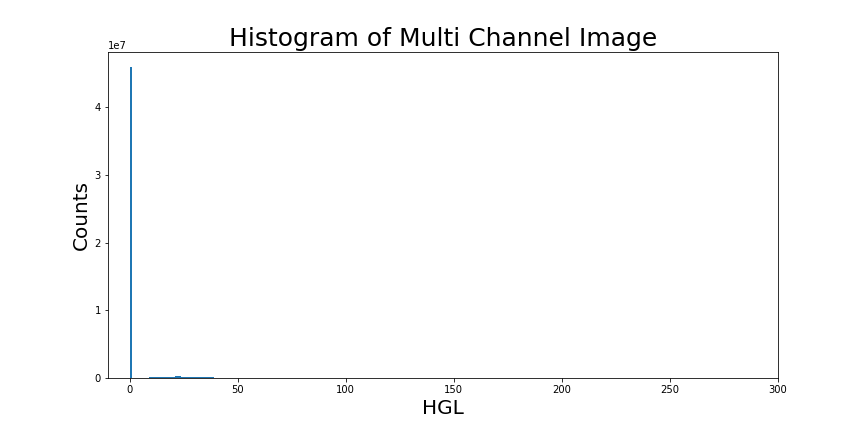
\includegraphics[scale=.5]{HistMC.png}
				\caption{Histogram of the multichannel image to cluster, we can clearly see the overrepresented cluster at $0$ GL}	\label{fig:ClusteringHistogram}
		\end{figure}
		
	An other problem may be the estimation of the correct number of clusters. k-means clustering requires a prior knowledge on the number of clusters which is a crucial choice. In our case the anatomical knowledge about the lung may help, since we can consider one cluster for each anatomical structure. In the end we have found that 5 clusters are an optimal choice, and the considered structures are the following: 
	\begin{itemize}
		\item Lung Parenchima;
		
		\item Edges;
		
		\item vessel surrounding bronchial structures;
		
		\item Ground Glass Opacities and consolidation;
		
		\item Bronchi.

	\end{itemize}

	
	We don't need a cluster to represent the background, since as I' ve said before the corresponding voxel aren't takes into account during the clustering.\\
	In the end a set of centroids for each subsamples was estimated and a second clustering was performed, to found the optimal centroids. 
	This process takes a lot of time, but once we have estimated the optimal centroid set, we haven't to repeat it.\\
	
	The whole step is summarized in the pseudocode in \figurename\,\ref{alg:training}.
		
		
	\begin{algorithm}
	
	\SetAlgoLined
	\DontPrintSemicolon
	
	\SetKwFunction{FSub}{shuffle\_and\_split}
	\SetKwFunction{Fk}{kmeans\_on\_subsamples}
	\SetKwProg{Fn}{Function}{:}{}
	
	\Fn{\FSub{$images,\, number of subsamples$}}{{
	
			images$\leftarrow$shuffle(images)\;
			output$\leftarrow$split(images, number of subsamples )\;
		}
		\textbf{return} $ output $ 
	}
	\textbf{End Function}

	\Fn{\Fk{$subsamples,\, number of centroids$}}{{
			
			centroids <- []\;
			\ForEach{$ Sub \in subsamples $}
			{
				center$\leftarrow$kmeans(sub, number of centroids)\;
				centroids$\leftarrow$append(center)
				
			}
		
		}
		\textbf{return} $ centroids $ 
	}
	\textbf{End Function}
	
	\KwData{CT scans with Extracted lung}
	\KwResult{Centroid matrix}
	
	\ForEach{$scan \in input\_scans$}{
	
		read the scan\;
		sample$\leftarrow$image\_array\;
	}

	sample$\leftarrow$ build\_multichannel(sample)\;
	subsamples$\leftarrow$shuffle\_and\_split(sample, number of subsamples)\;
	centroid\_vector$\leftarrow$kmeans\_on\_subsamples(subsamples, n\_centroids)\;
	centroid$\leftarrow$kmeans\_clustering(centroid\_vector, n\_centroids)\;
	
	\caption{Pseudo-code for the training script}\label{alg:training}
	
\end{algorithm}

	
\end{document}
	\begin{document}
	
	\subsection{Labeling}
	
	
	
	
	This is the last step of the pipeline and involves assigning of  each voxels to the cluster corresponding to the nearest centroids, in this way an hard segmentation is achieved.
	
	The script takes as input the CT scan after the lung extraction and it build the multichannel image as described before. After that it assigns each voxel to the cluster of nearest centroids, which is the one that minimize the distance : 
	\begin{equation}
		cluster = \arg\min_{S}  \sum_{i=1}^k \sum_{S} \| x - \mu_i\|
	\end{equation}
	
	where $x$ is the color vector of the voxel and $\mu$ is the $ith$ centroid. During this process the background is automatically assigned to the 0 label, by passing a mask which assume $0$ on the volxel background and $1$ for the other one. At the end of the assignment, only the cluster corresponding to GGO and CS is selected.
	To summarize the process, the pseudocode of the script is reported in algorithm\,\ref{alg:labeling}
	I've tested this algorithm on three different dataset, the results are described in the next chapter.
	
	\begin{algorithm}
		
		\SetAlgoLined
		\DontPrintSemicolon
		
		\SetKwFunction{Flabel}{imlabeling}
		\SetKwProg{Fn}{Function}{:}{}
		
		\KwData{CT scan to label, centroids}
		\KwResult{GGO label}
		
		image$\leftarrow$build\_multi\_channel\;
		\tcc{Compute distances and found the minimum}
		\ForEach{$c\in centroids $}
		{
			distances$\leftarrow\| image - c\|^2$\;
		}
		
		labels$\leftarrow\arg\min\,(distances)$\;
		
		\caption{Pseudo-code for the labeling script}\label{alg:labeling}
		
	\end{algorithm}
	

	The assignement process is performed by the \textsc{imlabeling} function, which takes care to assign the background to $0$, if the suitable parameter is passed.  The function is implemented as follows:
		
	\lstset{style=python}
	\begin{lstlisting}[language=python, caption=imlabeling, label=code:imlabeling]
		
	import numpy as np
	
	def imlabeling(image, centroids, weight = None) :


		if weight  is not None :
			distances = np.asarray([np.linalg.norm(image[weight != 0] -c, axis = 1) 
									for c in centroids])
		
			weight[weight != 0] = np.argmin(distances, axis = 0)
			return weight
		else :
			distances = np.asarray([np.linalg.norm(image -c, axis = 3) 
									for c in centroids])
			labels = np.argmin(distances, axis = 0)
			return labels
	
	
	\end{lstlisting}
	



	
	
\end{document}

	
	%Tuning of paramenters
	\documentclass{standalone}
\begin{document}
	\section{Optimization}
	
	During each step of the pipeline, we have to set different parameters, like the kernel size for median and std filter, as well as the number of centroids to use for the segmentation. In this section, I will briefly describe how each one of these parameters was optimized, to obtain the best segmentation performances.
	
\end{document}
	\documentclass{standalone}
\begin{document}
	\subsection{Estimation of the Number of Clusters}
	
	The designed algorithm for the centroids estimation is the k-means clustering that requires a prior knowledge about the number of clusters to use. This is very important since a bad choice will badly affect the whole segmentation results. In order to chose the proper number of clusters, I've consider two different sources of information: the anatomical knowledge about the lung and the internal variability of the lung.
	
	From anatomical knowledge about the lung, we can derive 5 clusters, corresponding to: 
	
	\begin{itemize}
		\item Lung Parenchima; 
		
		\item  Edges;
		
		\item Vessel surrounding bronchial structures;
		
		\item  Ground Glass Opacities and consolidation;
		
		\item Bronchi.
	\end{itemize}

	Notice that the background of the image is not considered as a cluster since it is removed from the segmentation for the reasons explained before.
	In order to verify that this number of clusters is the best one, I have considered the internal cluster variability.
	
	Clustering techniques try to group the data into different clusters  in order to maximize the difference between points in different clusters and to maximize the similarity within each cluster.  If the number of centroids is less then the clusters one, the similarity within each cluster is low. Increasing the number of centroids, will reduce reduce the internal variability till $0$ (if number of clusters is equal to the number of points). 
	This means that after a a certain point the diminishing of the internal variability is no more significant, since do not correspond to the good number of clusters but only to the increasing of their number.
	
	To found the correct number of clusters we are seek to for a number of clusters which still provides a small amount of internal variability. 
	
	To achieve this purpose, the clustering was repeated several times increasing the number of clusters and for each iteration the internal variability was measured by the sum of squares estimate error (SSE) : 
	\begin{equation}\label{eq:SumOfSquare}
		SSE = \sum (x_i - c_j)^2
	\end{equation}
	
	Once this task is completed, the results was printed in \figurename\,\ref{fig:ElbowCurve}. 
	
	\begin{figure}[h!]
		\centering
		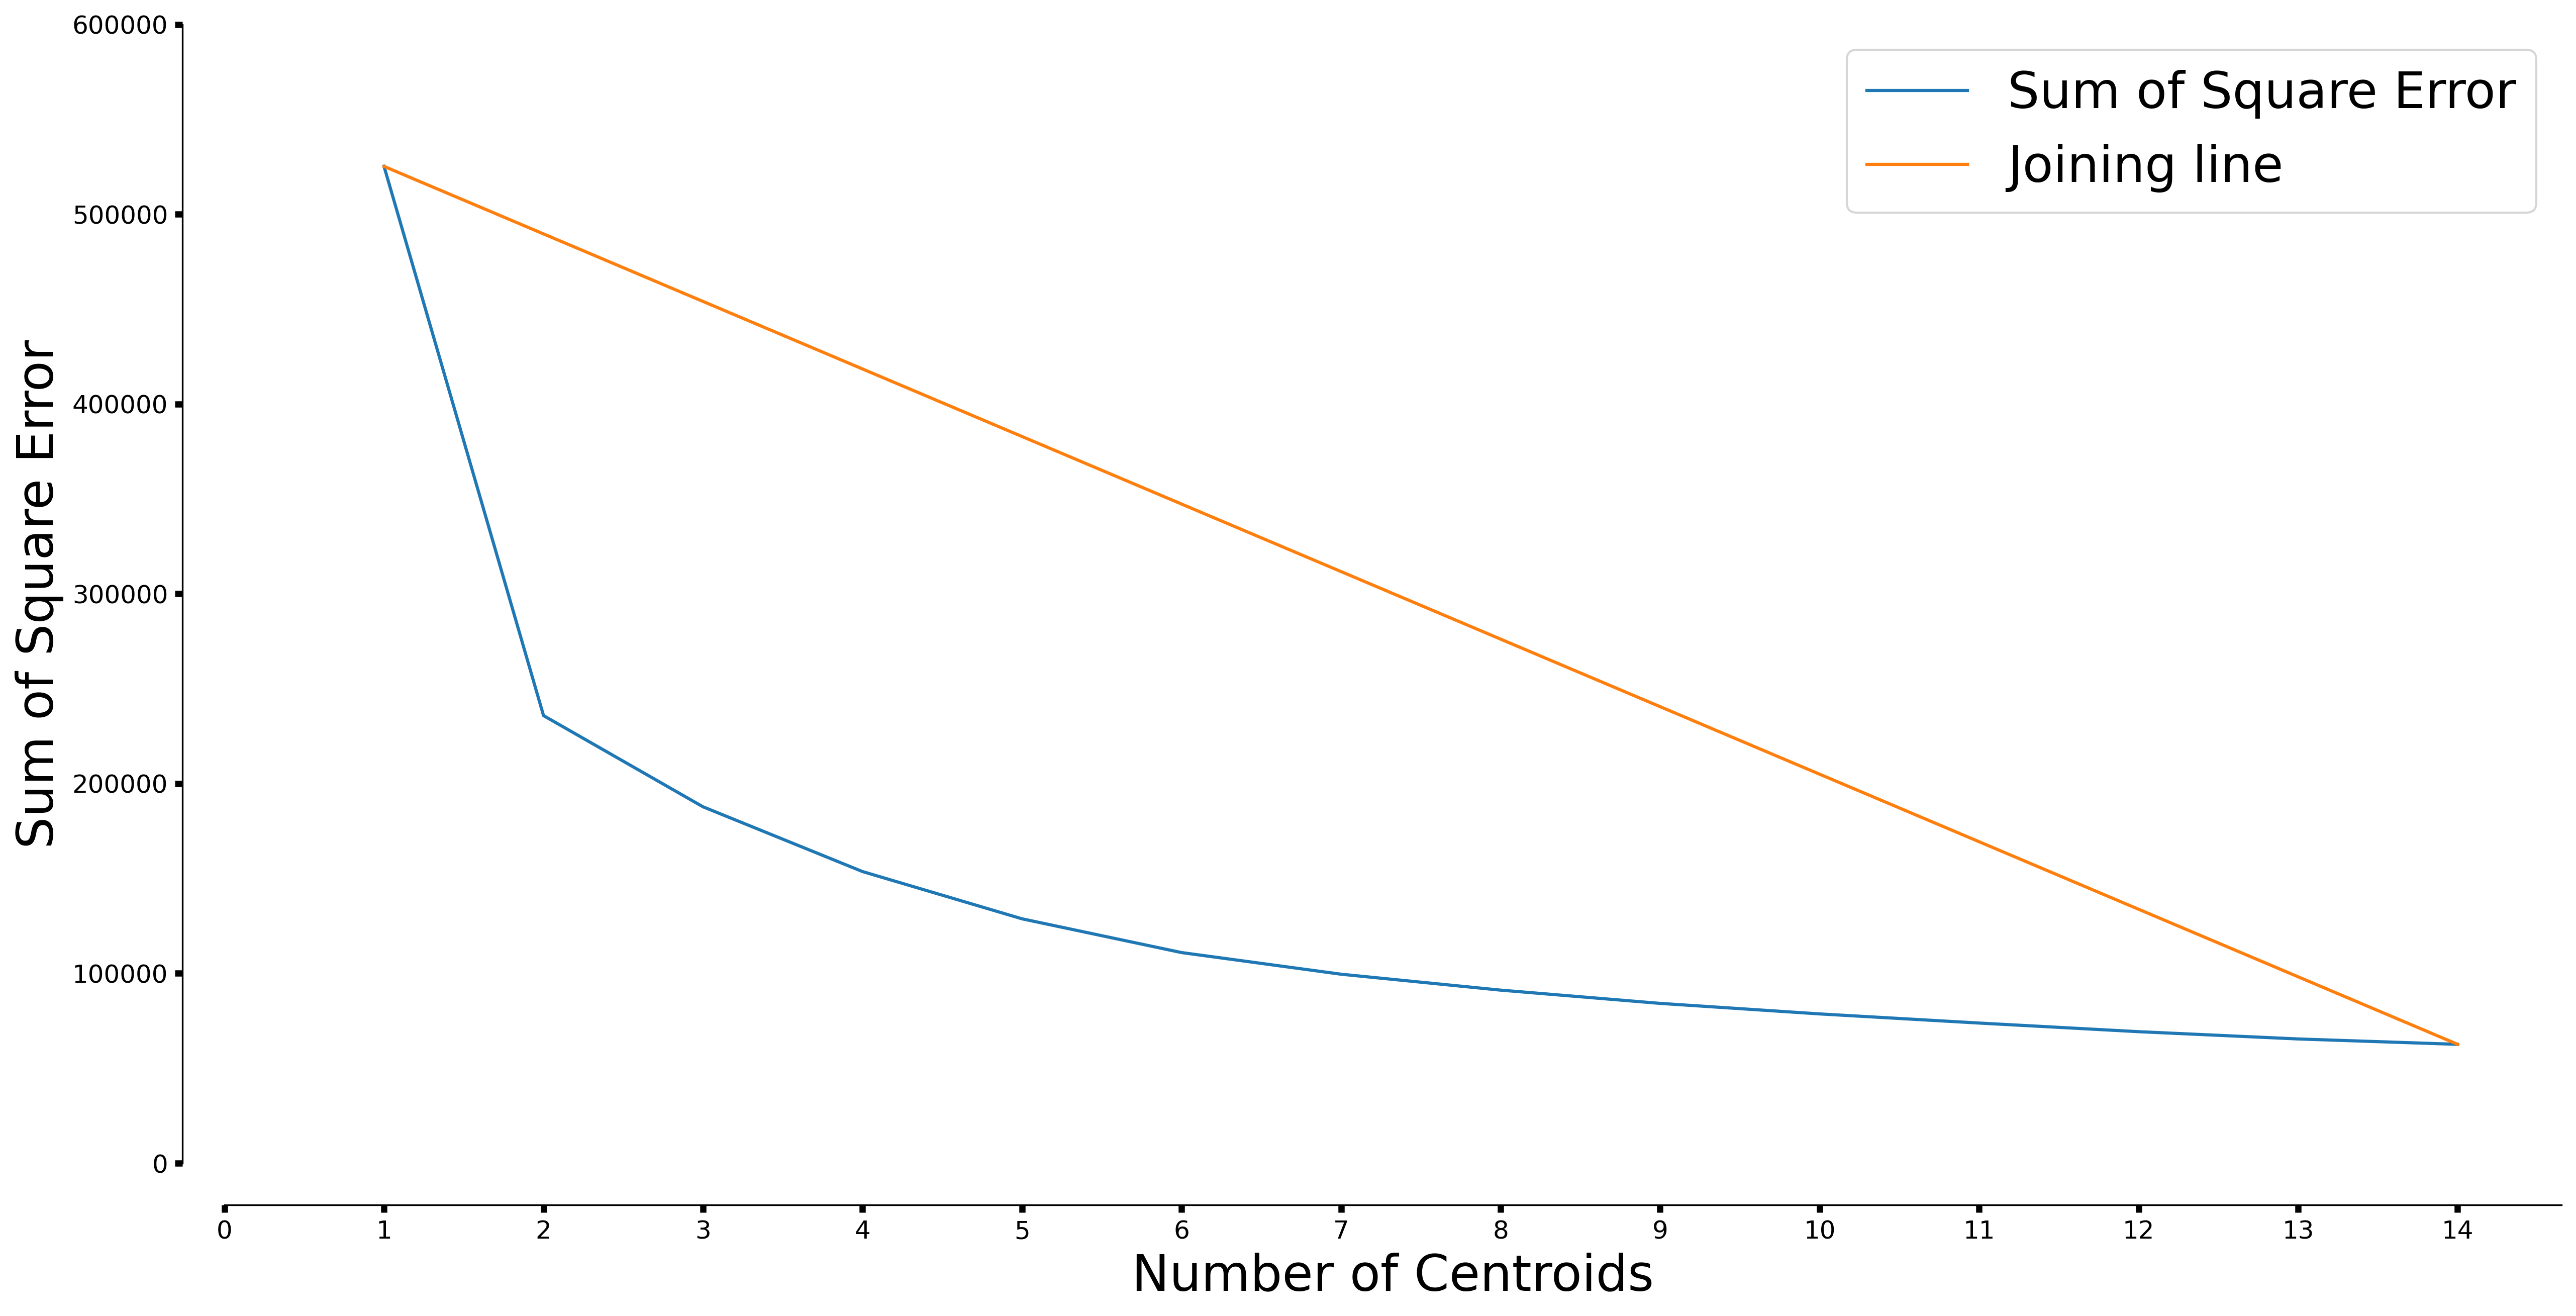
\includegraphics[scale=.3]{ElbowCurve.png}
		\caption{Intra-cluster variance vs the number fo clusters(blue); right joining firts and last point(orange). We can se the elbow shape of the graph; the elbow location in the one which maximize the distance between the right joining line and the elbow curve.}\label{fig:ElbowCurve}
	\end{figure}

	The optimal number of cluster is the one that corresponds to the elbow of the curve. It is difficult to find this feature from visually, I took the numerical value of the elbow considering the point which maximize the distance between the right joining the first and the last point.
	From this analysis I have found that the optimal number of clusters is $5$, which corresponds to the same that I have found considering the lung anatomy.
	
\end{document}
	\documentclass{standalone}
\begin{document}
	\subsection{Kernel Size Optimization}
	
	During the building of the multi channel image, we have to compute different image features, that requires the setting of different parameters, like median or standard filter kernel size. In order to achieve the best segmentation, we have performed an optimization step. This step aims to found the parameters that allows to obtain the best segmentation. 
	
	Notice that this process is not necessary and a good segmentation can be achieved also by setting this parameters manually.

	In order to perform the optimization, I've used \textsc{scikit-optimize}~\cite{skopt}, more specifically the gc\_minimize method.
	
	This method seek to perform a Bayesian optimization by using a Gaussian process to approximate an objective function. The function values are assumed to follow a multivariate Gaussian. The covariance of the function values are given by a GP kernel between the parameters. Then a smart choice to choose the next parameter to evaluate can be made by the acquisition function over the Gaussian prior which is much quicker to evaluate~\cite{skopt}.

	In the end an objective function is minimized. The used objective function is defined in algorithm\,\ref{alg:optimize} in which is also reported the whole minimization pseudocode. The used function seek to minimize $1 - IoU$ where the IoU(Intersection over Union) is computed between the output labels and a reference one.
	
	I 've decided to use the IoU instead of accuracy since the number of pixels concerning the labeled object would be very few against the number of pixels related to the background. Thus, the label would be a matrix with a large amount of zeros (background) and only few ones (object). In this case the standard metric functions have to consider an unbalanced number of samples; so the solution was to use the IoU which  measures the ration between the Intersection and Union of the output labels and the binary ground truth~\cite{PhDtheis}:
	\begin{equation}
		IoU = \frac{Area\,of\,Overlap}{Area\,of\,Union}
	\end{equation}
	
	
	\begin{algorithm}[h!]
	
		\SetAlgoLined
		\DontPrintSemicolon
		\SetKwRepeat{Do}{do}{while}%
		\KwData{Test scans, Ground Truth}
		
		\SetKwFunction{Obj}{objective}
		\SetKwProg{Fn}{Function}{:}{}
		
			
		\Fn{\Obj{$parameters, ref\_labels, CT\_scan$}}{{
				
				$labels$ $\leftarrow$ segment($CT\_scan$)\;
				iou = IoU($labels$, $ref\_labels$)\;
			}
			\textbf{return} $ 1 - iou $ \;
		}
		
		
		$best\_parameters\leftarrow$gc\_minimize(objective, n\_calls, n\_random\_init)\;
		
			\caption{Parameter Optimization Algorithm}\label{alg:optimize}
	\end{algorithm}
		
		
	This process allows to optimize the parameters in order to obtain the best results as possible. As reference labels I've used the ones valuated as gold standard from expert radiologist.
	
	This procedure allows only to tune the parameters for a better segmentation, but the learning process remains unsupervised.

\end{document}
	
	

\end{document}
\documentclass{standalone}
\begin{document}


	\documentclass{standalone}
\begin{document}
	\chapter{Results}
	

	The developed pipeline was trained and tested on three datasets (Sant'Orsola, ZENODO and MOSMED), described in the first section. 
	After that I will discuss the segmentation performances. The main method for the evaluation were a quantitative comparison whit a gold standard segmentation, made and validate by $5$ experts with at least $2$ years of experience. In collaboration with Sant'Orsola, the pipeline results were compared with some semiautomatic segmentation by a blind evaluation made by experts.
	As a control also segmentation on healthy patient were made, in order to ensure that no lesion were detected. This kind of segmentation was useful also to find the main source of errors. 
\end{document}
	
	%Dataset Description
	\documentclass{standalone}
\begin{document}
	\section{DataSet Description}
	
	This section is dedicated to the description of the datasets used for the developing and test of the pipeline. The description includes general image characteristics and some metadata. If within the datasets are provided also some manual annotation, also the segmentation masks are described. 
\end{document}
	\documentclass{standalone}
\begin{document}
	\subsection{Sant'Orsola}
	
	Sant'Orsola data was the ones mainly considered in this work. It consist into 83 anonimyzed CT scans from $83$ different patients affected by COVID-19 and $8$ scans from healthy controls. 
	Within these scans, also manual annotation were provided. These annotations were obtained with a semi-automatic approach. The built of each annotation may requires several hours.
	
		The series are distributed as follows: 
	\begin{table}[h!]
		\centering
		\begin{tabular}{|c|c|}
			\hline
			\textbf{Property}   		&	\textbf{Value} \\ \hline
			Number of Scans 			& 83			   \\ 
			Distribution by sex(M/F/O)  		& 66.3/33.7/0    \\
			Distribution by age(min/median/max) & 35/60/89	\\ \hline
		\end{tabular}
	\end{table}
	
	
	For $5$ scans were provided also other semi-automatic segmentations. These segmentation were obtained by refining the initial segmentation of a certified software. The building of these labels has required several days. In the end this results are validated by $5$ experts with at least $2$ years of experience. These $5$ segmentation represents the gold standard used as ground truth.
	
\end{document}
	\documentclass{standalone}
\begin{document}
	\subsection{MOSMED}
	
	MosMed is a dataset which contains 1110 anonymized CT scan of human lung from both patients affected by COVID-19 in several stages fo the disease, and healthy controls. A small subset of this scans is labeled. The scans are obtained between 1st March and 25th of april 2020 by different Russian hospitals. This dataset was born with educational and AI developing purposes. The studies are divided into 5 cathegories, from healty patients to the most severe cases. Each scan of the dataset is saved in \emph{.nfti} format and during the conversion from the original dicom series only 1 image every 10 was preserved.
	The resulting dataset have the following characteristics: 
	
	\begin{table}[h!]
		\centering
		\begin{tabular}{|c|c|}
			\hline
			\textbf{Property} 		   				   & \textbf{value}	  \\ \hline
			Number of Scans 		   				   & 1110             \\ 
			Distribution by sex(M/F/O) 				   & 42/56/2          \\
			Distribution by age(min/median/max)		   & 18/47/87         \\
			Number of studies in each cathegory		   & 254/648/125/45/2 \\ \hline
			
		\end{tabular}
	\end{table}

	The CT scans are organized into 5 cathegories, depending on the percentage of the involved lung volume : 
	\begin{table}[h!]
		\centering
		\begin{tabular}{|c|c|}
			\hline
			\textbf{Class} & \textbf{Description} \\ \hline
			CT-0		   & Normal  lung tissues \\
			CT-1		   & presence of GGO, lung parenchima involved less than $25\%$ \\
			CT-2		   & GGO, involvement of lung parenchima in $25 - 50\%$ \\
			CT-3		   & GGO and consolidation, involvement of lung parenchima in $50 - 75\%$ \\
			CT-4		   & GGO, consolidation and reticular changes, lung parenchima involved more than $75\%$\\ \hline
		\end{tabular}
	\end{table}

	Of these five cathegories only $50$ annotations are available, mostly involving only the patients of CT-1 groups. Scans have been annotated by the experts of Research and Practical Clinical Center for Diagnostics and Telemedicine Technologies of the Moscow Health Care Department.
\end{document}
	\documentclass{standalone}
\begin{document}
	\subsection{ZENODO}
	This dataset consists into $20$ CT scans of patients affected by COVID-19, labeled by two expert radiologists and verified by  third one. 
	The anatomic structures labeled are the left and right lung and the infections regions. 
	Each files is in nifti format and no metadata were available.
	
	Unfortunately only an half of the scans are in HU, the remaining are in 8-bit gray scale, which is not suitable to verify the pipeline since requires it as input an image in HU.
\end{document}
	
	%Timing
	\documentclass{standalone}
\begin{document}
	\section{Time Performances}
	As I've said before the time performances are a relevant parameter of this pipeline. In this section I will discuss the segmentation time.  Since for this work I've to segment several scans (over than $100$), I've performed the  two main step (lung extraction and labeling) seprately, and compute the time segmentation time for each slice and phase. The timing for the training step was not measured since this step is performed only once, so doesn't affect the total segmentation time.\\
	The time performances are measured by performing the segmentation on the DIFA servers.\\
	
	In \figurename\,\ref{figTiming_lab} I've plotted the times of the labeling  step for each scan versus the number of slices of the scan. As we can see the timing increase linearly with the number of slices. In order to find the segmentation time for the single slice, I've performed a linear fit, the desidered time will correspond to the angular coefficient.From this analysis I've measured that the segmentation time $0.074\,sec$ for each slice of the CT scan. 
	\begin{figure}[h!]
		\centering
		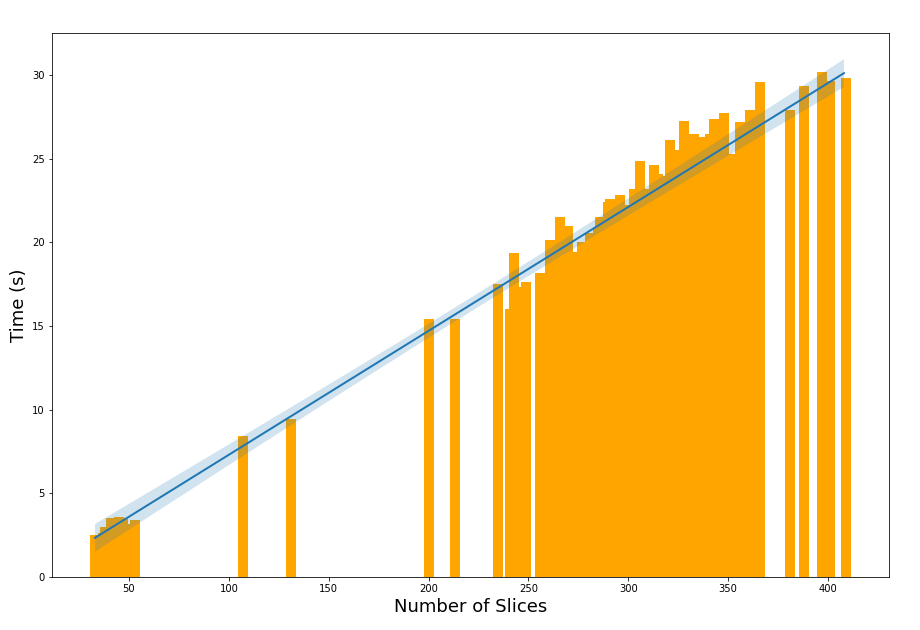
\includegraphics[scale=.75]{Timing_lab.png}
		\caption{Total labeling time vs number of slice for each scan of each dataset}	\label{fig:Timing_lab}
		
	\end{figure}
	
\end{document}


	
	% Accuracy
	
	\documentclass{standalone}
\begin{document}
	
	\section{Accuracy}
	
	
	In this section I will comapare the pipeline segmentation against the annotations. 
	The pipeline was trained over $10$ CT scans, carefully selected from the available datasets. This ensure a balanced cluster representation. 
	Using this set of centroids I have segmented the CT scans of the $3$ available datasets, and match the  achieved results whit the annotations, when available.
	
	The automatic pipeline was run on the servers of the Department of Physics and Astronomy (DIFA), and its able to achieve a segmentation in less than $2$ minutes. 
	
	\begin{figure}[h!]
		\centering 
			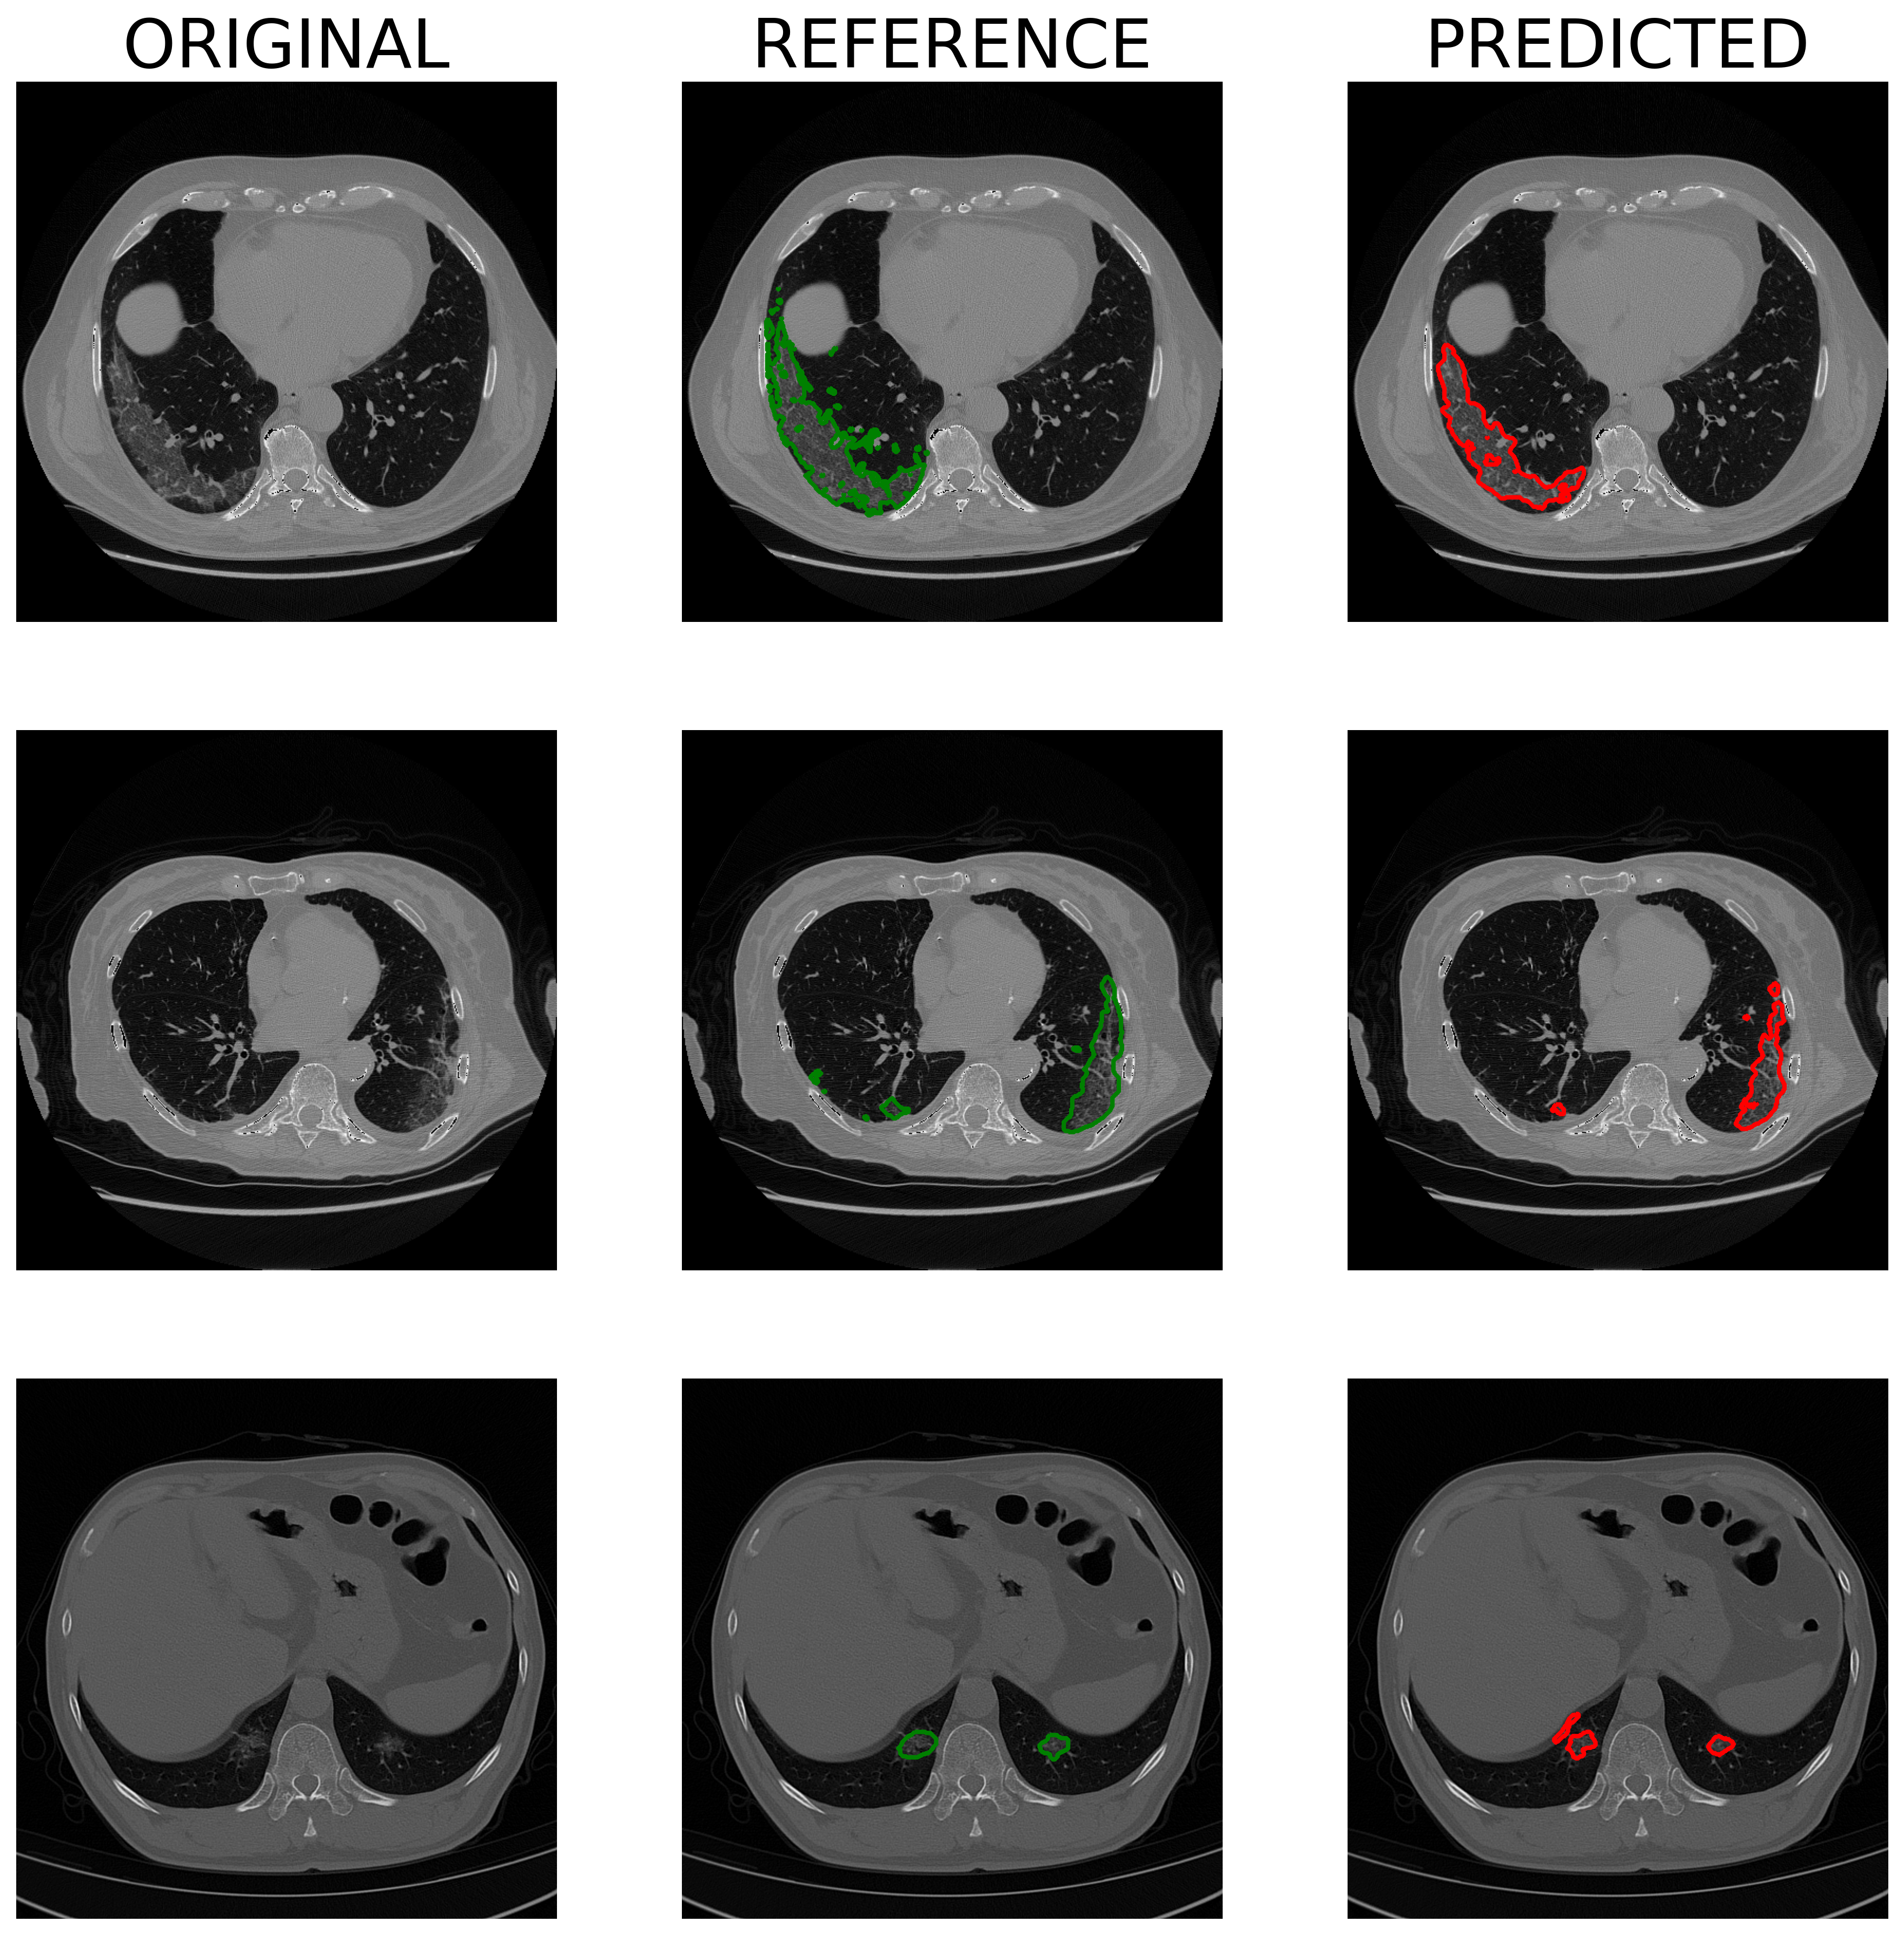
\includegraphics[scale=.2]{Results1.png}
			\caption{Comparison between the achieved segmentation (red) and the reference (green). We clearly see that the GGO ans CS areas are well identified and segmentented}\label{fig:Results}
	\end{figure}

	In \figurename\,\ref{fig:Results} I've reported a comparison between the achieved results and the reference segmentation. We an observe that GGO and CS areas are correctly segmented. 
	
	\begin{figure}[h!]
		\centering
			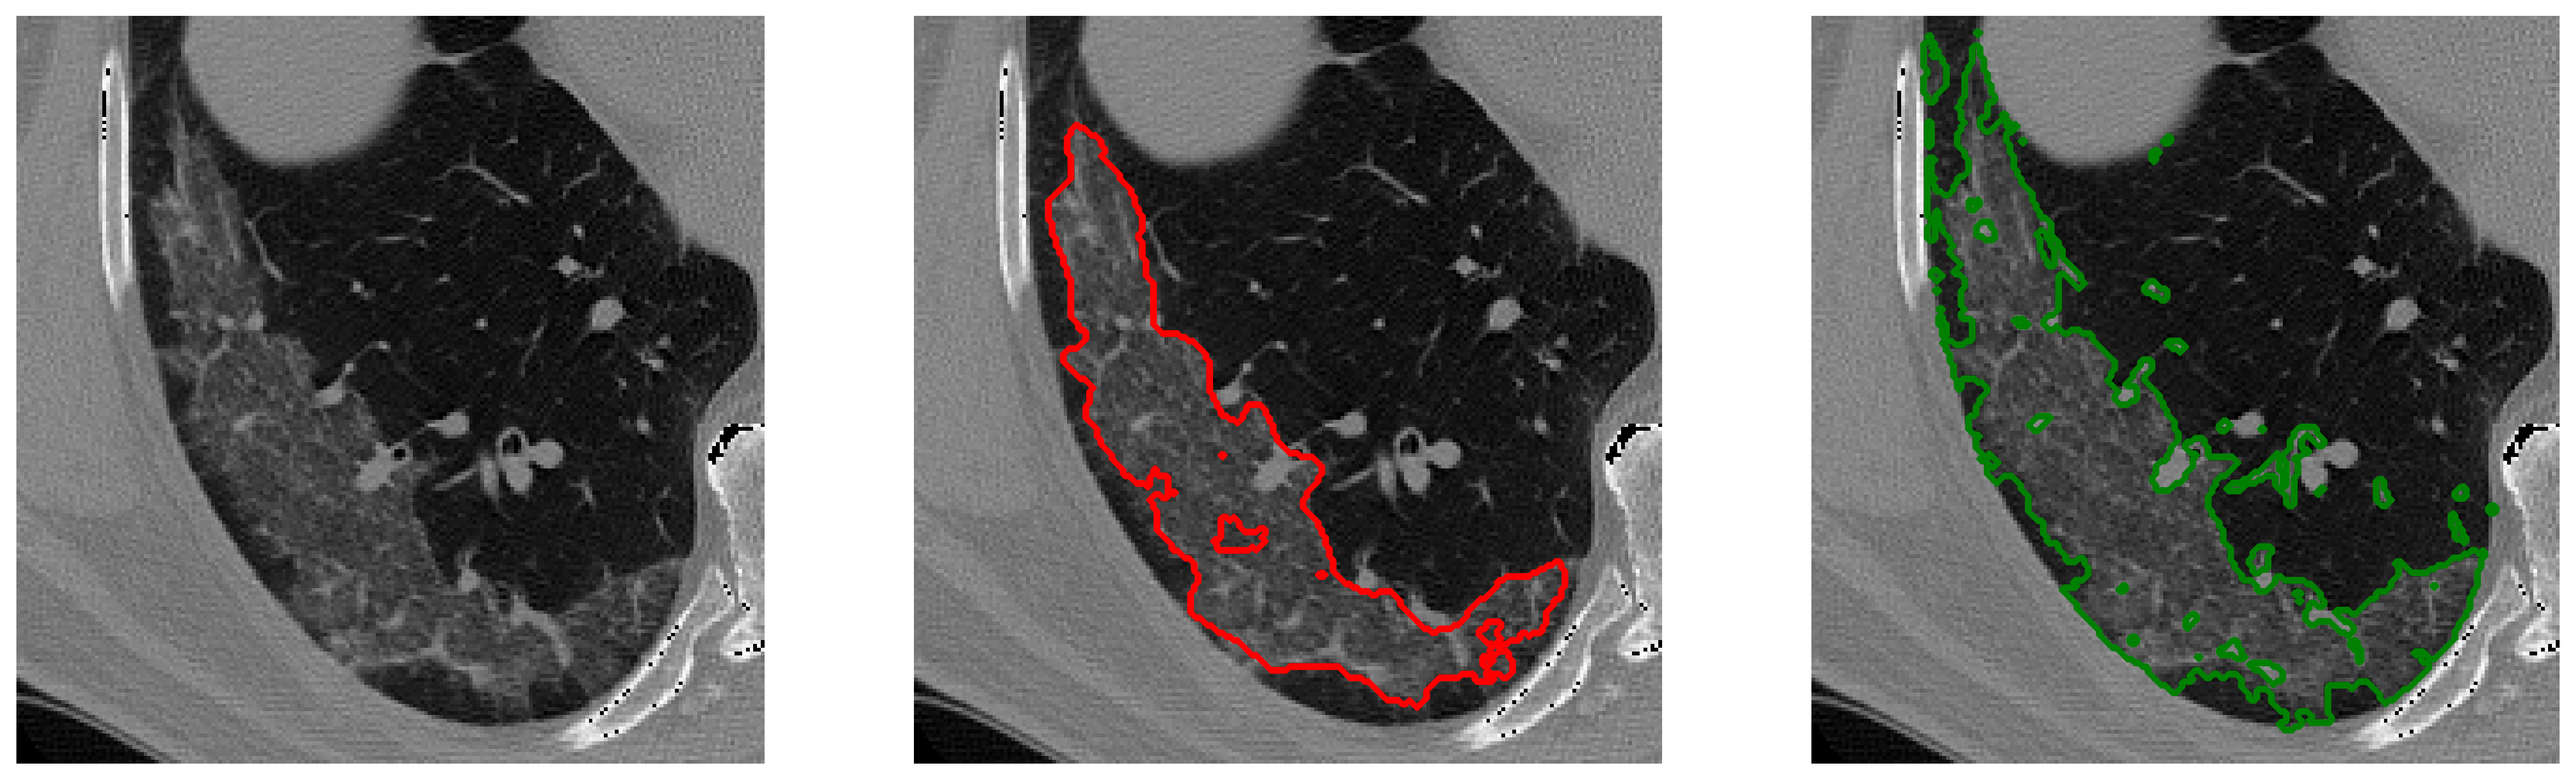
\includegraphics[scale=.37]{zoom.png}
			\caption{Focus on lesion area. From left to right we can observe the original image, the predicted lesion areas and the reference one. We can observe that the annotation  identify a larger area. The annotation identify also some spots outside the lesions which seems to be healthy tissue}\label{fig:zoom}
	\end{figure}
	
	
	In \figurename\,\ref{fig:zoom} I have reported a zoom on the identified lesions areas. As we can see both the pipeline segmentation and the annotations correctly identify the areas of interest. We can observe that in the semi-automatic method there are some spot which do not seem to belong to a lesion area. Moreover the automatic segmentation seems to identify a lesions with less areas.
	
	
	In \figurename\,\ref{fig:3Dlabel} I've reported a 3D rendering of the lung, with the identified lesions. In pink we can see the manual annotation, in green the segmentation achieved by the pipeline. From these images is more clear that the total estimated volume is different between the two methods. In particular the annotations incorporates a larger volume than the pipeline segmentation.
	
	\begin{figure}[h!]
	
		\centering 
			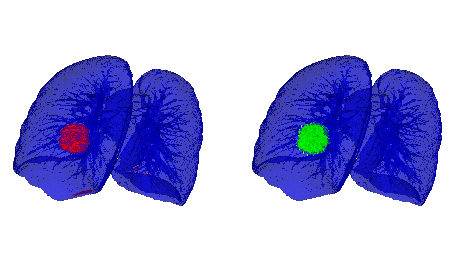
\includegraphics[scale=.4]{3Dlesion.png}
			\caption{3D representation of lesions. From left to right the manual annotation (pink) and the pipeline segmentation (green). We can observe that the segmented size of the area is different.}\label{fig:3Dlabel}		
	\end{figure}
	
	
	In order to assess the quality of the achieved segmentation, I've used two different method. 
	
	First of all I've compared both the pipeline segmentation and the annotations with a gold standard. In this way I was able to measure the proportion of the areas correctly identified.
	
	After that the segmentation was submitted to five experts in order to made a blind evaluation, comparing the pipeline segmentation with the reference one.
	
	In the section below I will describe these kind of measures.
	
	
\end{document}
	\begin{document}
	\subsection{Healty Control}
	
	In this part I will discuss the results of the segmentation of healthy controls. The segmentation was performed on $8$ scans, by using the same method described before.  In  
\end{document}
	\documentclass{standalone}
\begin{document}
	\subsection{Zenodo and Mosmed}
\end{document}
	\documentclass{standalone}
\begin{document}
	\subsection{Comparison with Manual Annotations}
	
	In order to check the pipeline performances I have compared the  obtained segmentation with the manual annotation. To do that I have considere $5$ scans from the sant'Orsola dataset for which was available also a ground truth. This ground truth consist in an semi-automatic segmentation made with a certified software and refined by an expert with more than $5$ years of experience. After that the segmentation was validated by $5$ experts with at least one year of experience. This segmentation process takes several days. 
	
	In order to compare annotation and pipeline segmentation, I have computed the \emph{sensitivity} and \emph{specificity}: 
	
	\paragraph{Sensitivity} refers to the ability to correctly detect ill areas. It is defined as total number of voxels correctly classified as opacities (True Potitives), over the total number of positives (True Positives + False Negatives) : 
	\begin{equation}\label{eq:sensitivity}
		Sensitivity : \frac{True Positive}{True Positive + False Negatives}
	\end{equation}

	\paragraph{Specificity} relates to the  ability to correctly reject healthy areas. Is defined as the number of rejected pixels(True Negative) against the total number of healthy areas (True Negative + False Positives) : 
	\begin{equation}
		spcificity : \frac{True Negative}{True Negative + False Positives}
	\end{equation}

	I have displayed the results in table\,\ref{tab:Measures}. 
	
		\begin{table}[h!]
		\centering
		\begin{tabular}{|c|c|c|c|c|}
			\hline
			\multirow{2}{*}{}		  & \multicolumn{2}{c|}{Predicted} & \multicolumn{2}{c|}{Annotation} \\ \hline
						& Sensitivity & Specificity	 		& Sensitivity & Specificity		 \\ \hline
			Patient 1	& $0.412$	  &	$\sim 1.00$			&	$0.676$	  &	$ 0.999$ 		 \\ 
			Patient 2	& $0.399$	  & $\sim 1.00$ 		&	$0.698$	  & $ 0.995$		 \\
			Patient 3	& $0.570$	  &	$\sim 1.00$			&	$0.653$	  & $ 0.999$		 \\
			Patient 4	& $0.512$	  & $\sim 1.00$			&	$0.325$	  & $ 0.999$		 \\
			Patient 5 	& $0.628$	  & $\sim 1.00$			&	$0.974$	  &	$ 0.999$		 \\ \hline
		\end{tabular}\caption{Sensitivity and Specificity for the pipeline segmentation and annotation. As a ground truth was used a sem-automatic segmentation made and evaluated by $5$ experts with at least $2$ years of experience.}\label{tab:Measures}
		
	\end{table}

 	The first thing we can notice is that both the method have an high specificity. That means that  they rarely gives positives results for healthy regions (lower type I error rate): means that there is a low probability to obtain false positives. 
 	The situation changes when we consider specificity. We can see that the annotation have achieved a better sensitivity than the pipeline. That means that they rarely gives negative results for GGO regions (lower type II error rate). However this coefficient does not takes into account the rate of false positives, that means we cannot ensure that the detected GGO areas are really sick.
 	
 	This in agreement to the fact that, generally , the operator tends to include large lesion areas. However that is not always the case, since will depends to operator that performs the segmentation.
 	
 	
 	\begin{figure}[h!]
 		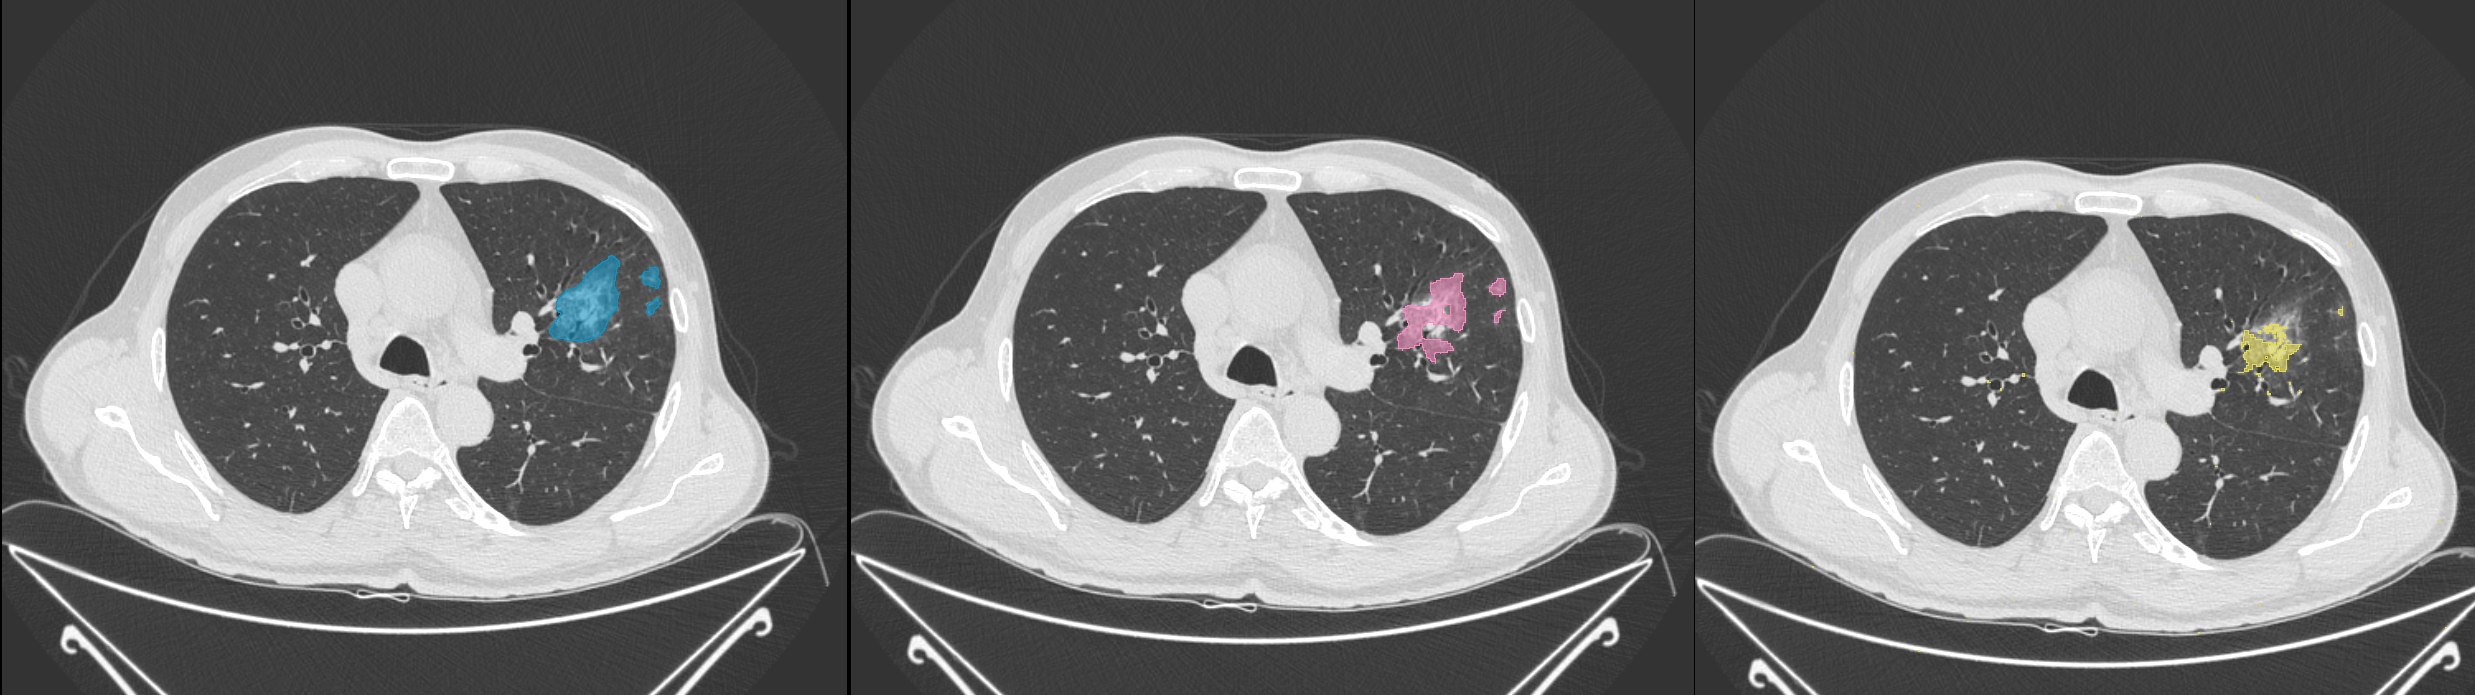
\includegraphics[width=\linewidth, height=.25\textheight]{GTCOM2.png}
 		
 		\caption{Comparison between the ground truth (blue), the pipeline segmentation (pink) and the manual annotation (yellow). We can see that the segmentation obtained by the automatic pipeline is better that the one of the manual annotation.}\label{fig:conf2}
 	\end{figure}
 
 	In \figurename\,\ref{fig:conf2} I have reported the results of the segmentation of Patient $4$. We can see the ground truth (blue), the pipeline segmentation (pink) and the annotation (yellow). In this case we can see that both the pipeline and the annotation correctly identified the lesion areas. However we can see that the annotation is missing a lot of lesion. On the other hand the segmentation achieved by the pipeline seems to cerrectly segment the whole areas. 
 	
 	\begin{figure}[h!]
 		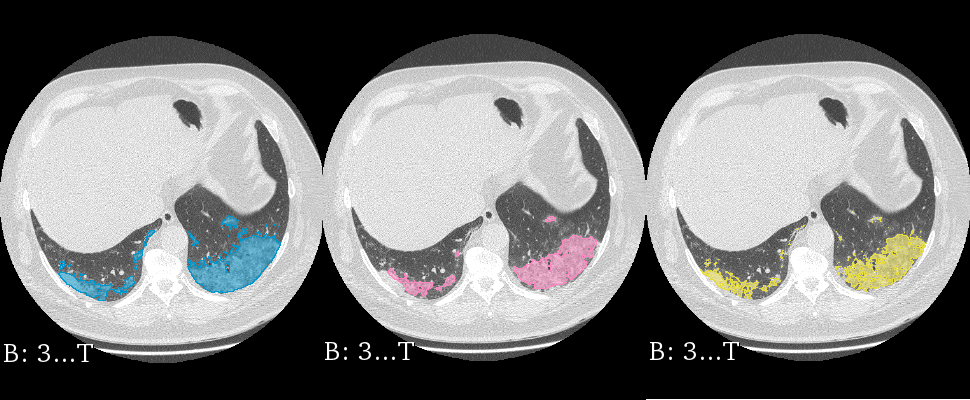
\includegraphics[width=\linewidth]{GTCOMP1.png}
 		
 		\caption{Comparison between the ground truth (blue), the pipeline segmentation (pink) and the manual annotation (yellow). We can see that the GGO an CS areas are correctly identified.}\label{fig:conf1}
 	\end{figure}
 
 	In \figurename\,\ref{fig:conf1} vI have reported the segmentation results for the third patient. We can see the ground truth (blue), the pipeline segmentation (pink) and the annotation (yellow). Also in this case the pipeline seem to correctly identify the opacity. In this case also the annotation seems to be in agreement with the ground truth.
 	
 	\begin{figure}[h!]
 		\centering
 		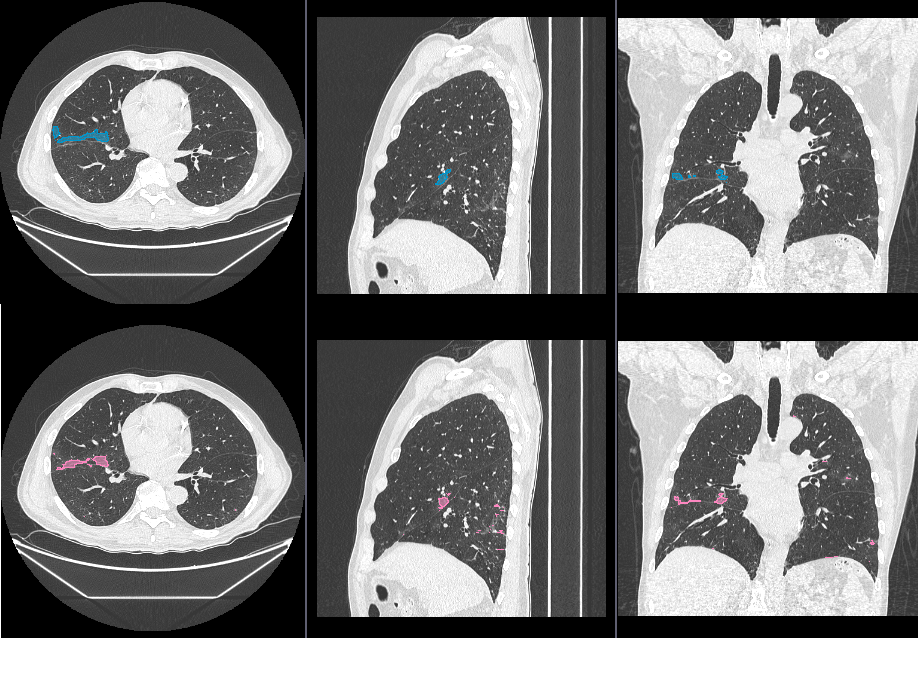
\includegraphics[width=.8\linewidth]{PATIENT1.png}  
 		\caption{Comparison between the gold standard segmentation(blue) and the pipeline results(pink) for axial, sagittal and coronal view of a patient with a low involvement of lung volume. We can see that te main lesion areas are identified, even if an underestimation of the total volume is present together with some small misclassified points.}\label{fig:pat1}
 	\end{figure}
 	
 	Up to now I have considered only two case in which the GGO and CS regions are well defined with high contrast respect to healthy lung volume. In \figurename\,\ref{fig:pat1} I have reported axial, sagittal and coronal view of the ground truth (blue) and pipeline segmentation (pink) for the first patient. This patient presents a low volume of GGO and CS. Moreover the identification is difficult due to the low contrast between lesion areas healthy lung volume. As we can see the lesion areas are correctly identified even if some misclassified regions are presents. 
 	
 	In the end I have to point out that the annotation and ground truth, since are obtained by semi-automatic method, requires  trained personnel and several hours (the first) or days (the seconds).  
 	
	

\end{document}
	\documentclass{standalone}
\begin{document}
	\subsection{Expert Evaluation}
	
	One control that was made to check the quality of the achieved segmentation, was a blind expert evaluation. We have randomly select $40$ patients from the three dataset and organized the scans as follows: \\
	For each patient we have displayed, slice by slice,  two images: the scans with the pipeline segmentation(the one to test), and the manual labels provided within the dataset (control) as in \figurename\,\ref{fig:Blind}.
	
	\begin{figure}[h!]
		\centering
			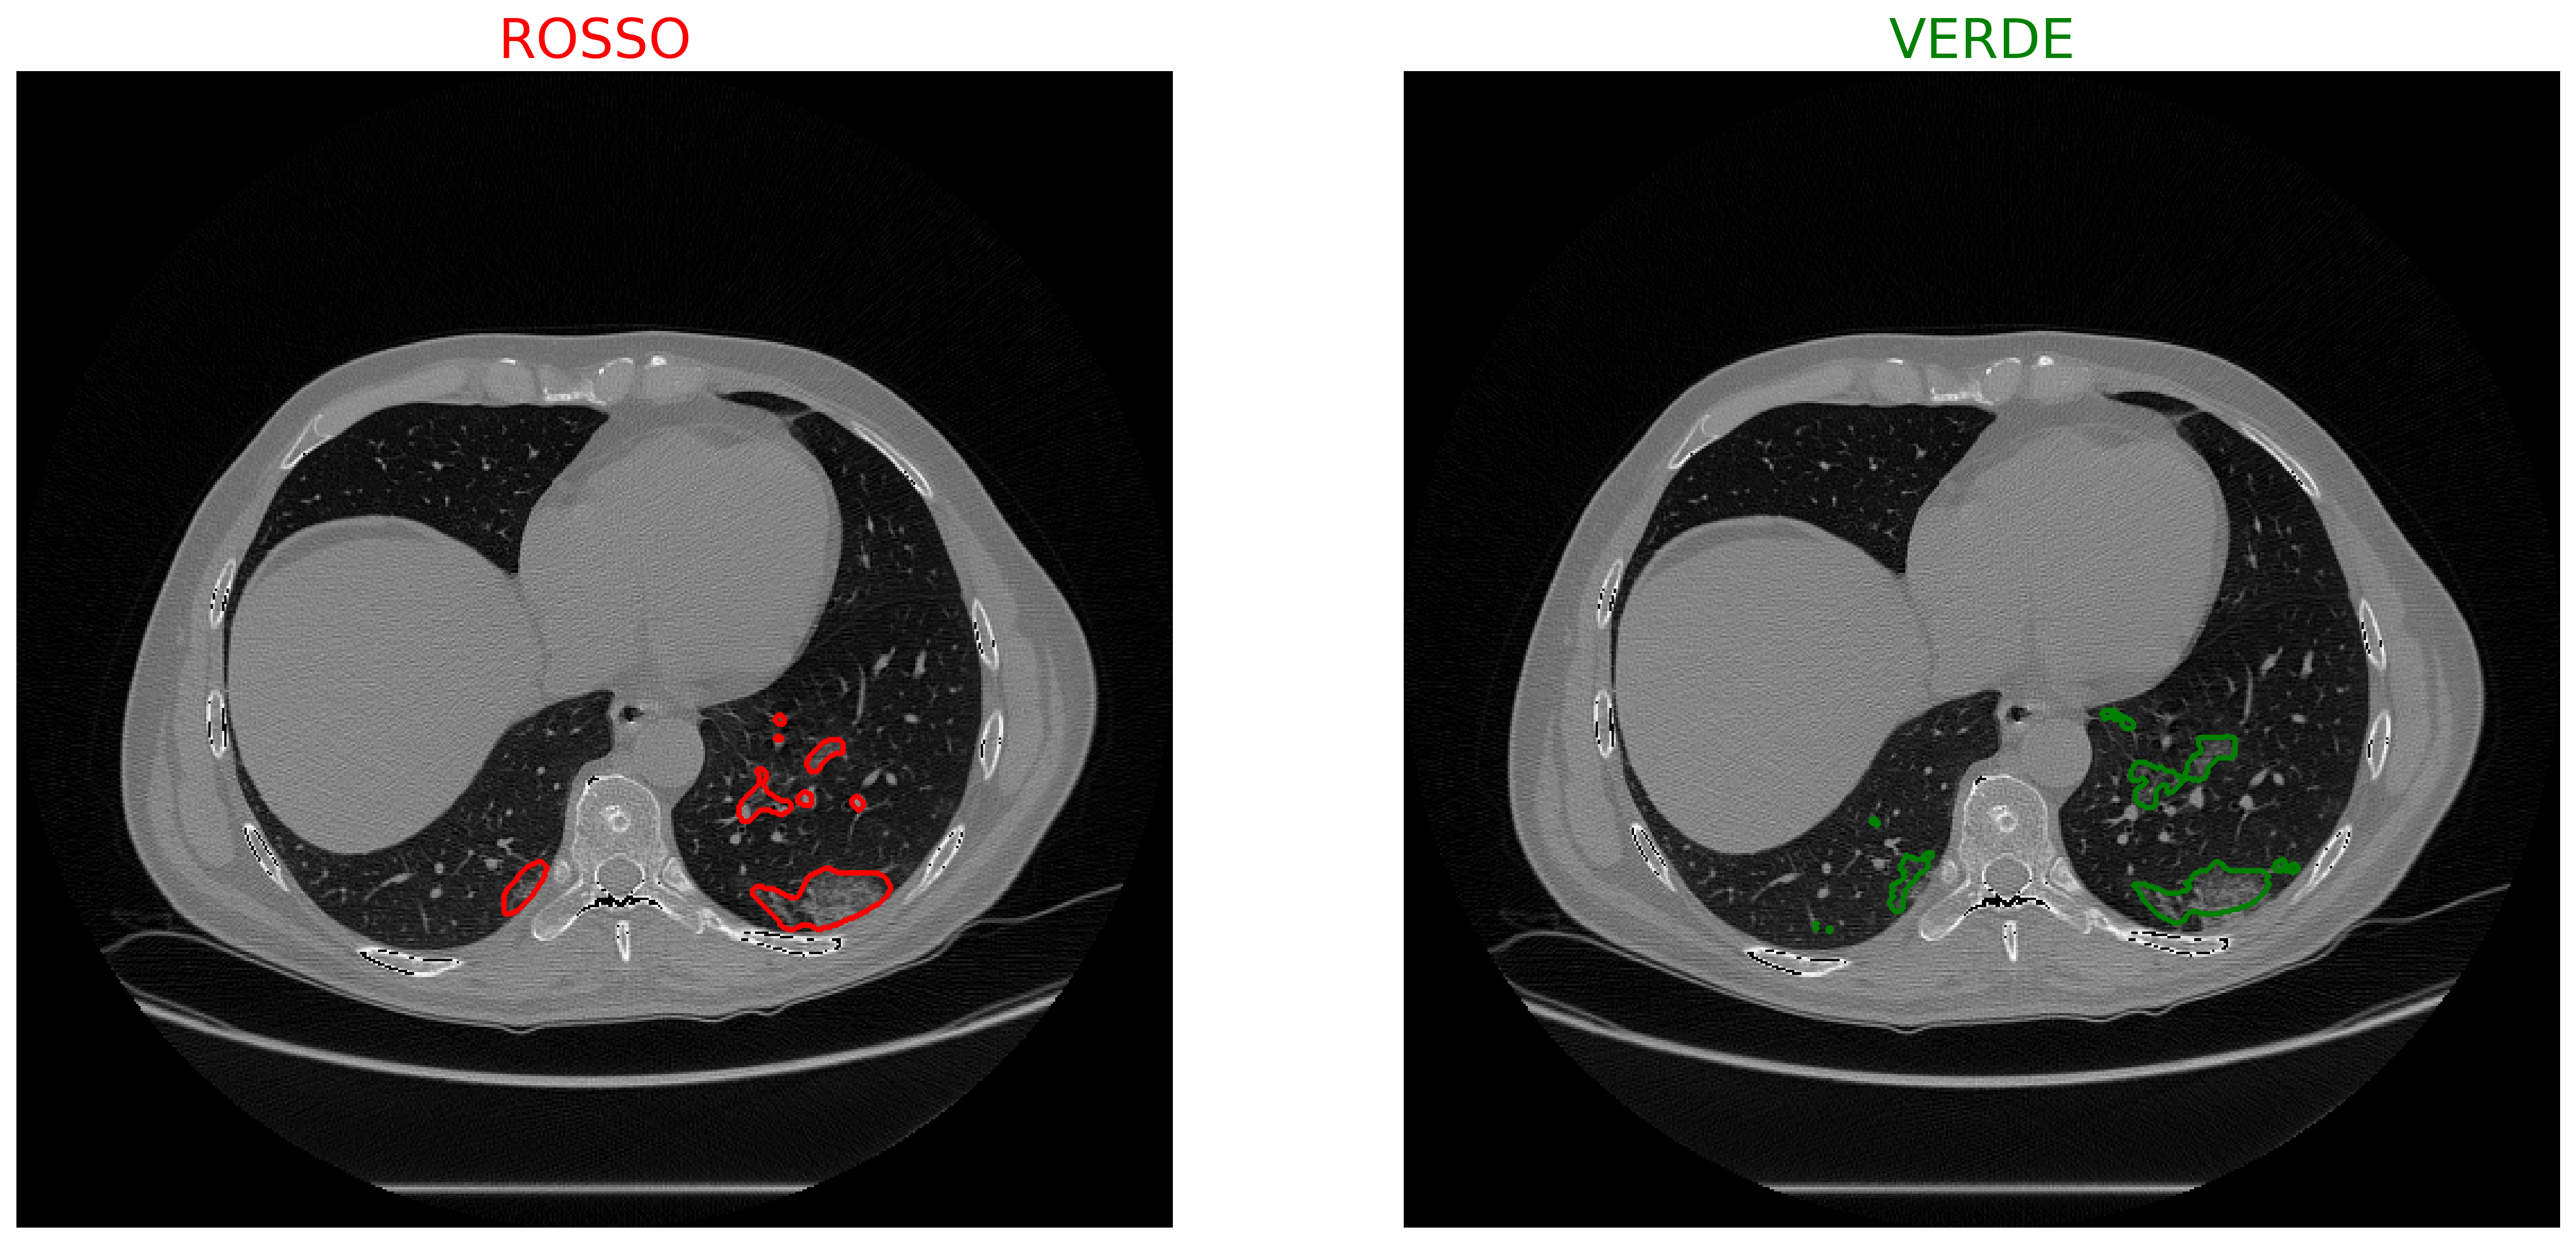
\includegraphics[scale=.3]{BlindEval.png}
			\caption{Example of comparison submitted to the experts. The two images report the segmentation of the same slices achieved with two different techniques: Manual and pipeline. Was asked to the expert to decide which one is better, without knowing which technique is used to obtain the segmentation.}\label{fig:Blind}
	\end{figure}

	The scans, organized in this way, was evaluated by experts, to which has been asked to decide, slice by slice, which segmentation is better or if the quality is equal.\\ The core of this method is that the expert doesn't know which scan correspond to a specific segmentation technique.  In order to ensure that, the order of segmentation was shuffled between patients.

	
\end{document}
	\documentclass{standalone}
\begin{document}
	\subsection{Discussion}
\end{document}
\end{document}


% conclusions
\documentclass{standalone}
\begin{document}

\chapter{Conclusions}

\end{document}

\printbibliography



\end{document}
